% **************************************************
% Document Class Definition
% **************************************************
\documentclass[%
    paper=A4,               % paper size --> A4 is default in Germany
    twoside=true,           % onesite or twoside printing
    openright,              % doublepage cleaning ends up right side
    parskip=full,           % spacing value / method for paragraphs
    chapterprefix=true,     % prefix for chapter marks
    11pt,                   % font size
    headings=normal,        % size of headings
    bibliography=totoc,     % include bib in toc
    listof=totoc,           % include listof entries in toc
    titlepage=on,           % own page for each title page
    captions=tableabove,    % display table captions above the float env
    draft=false,            % value for draft version
]{scrreprt}%


% **************************************************
% Setup YOUR thesis document in this file !
% **************************************************
% !TEX root = my-thesis.tex


% **************************************************
% Files' Character Encoding
% **************************************************
\PassOptionsToPackage{utf8}{inputenc}
\usepackage{inputenc}


% **************************************************
% Information and Commands for Reuse
% **************************************************
\newcommand{\thesisTitle}{Mastering Divserse Computer Games using Generation Based Learning}
\newcommand{\thesisName}{Manuel Esberger}
\newcommand{\thesisSubject}{Bachelor Thesis}
\newcommand{\thesisDate}{September xx, 2018}
%\newcommand{\thesisVersion}{}

\newcommand{\thesisFirstReviewer}{Jane Doe}
\newcommand{\thesisFirstReviewerUniversity}{\protect{Clean Thesis Style University}}
\newcommand{\thesisFirstReviewerDepartment}{Department of Clean Thesis Style}

\newcommand{\thesisSecondReviewer}{John Doe}
\newcommand{\thesisSecondReviewerUniversity}{\protect{Clean Thesis Style University}}
\newcommand{\thesisSecondReviewerDepartment}{Department of Clean Thesis Style}

\newcommand{\thesisFirstSupervisor}{Univ.Prof. Dr. Allan Hanbury}
%\newcommand{\thesisSecondSupervisor}{}

\newcommand{\thesisUniversity}{\protect{Vienna University of Technology}}
\newcommand{\thesisUniversityDepartment}{Faculty of Informatics}
\newcommand{\thesisUniversityInstitute}{xxxx}
\newcommand{\thesisUniversityGroup}{xxxx}
\newcommand{\thesisUniversityCity}{Vienna}
\newcommand{\thesisUniversityStreetAddress}{Karlsplatz 13}
\newcommand{\thesisUniversityPostalCode}{1040}


% **************************************************
% Debug LaTeX Information
% **************************************************
%\listfiles


% **************************************************
% Load and Configure Packages
% **************************************************
\usepackage[english]{babel} % babel system, adjust the language of the content
\PassOptionsToPackage{% setup clean thesis style
    figuresep=colon,%
    sansserif=false,%
    hangfigurecaption=false,%
    hangsection=true,%
    hangsubsection=true,%
    colorize=reduced,%
    colortheme=bluegreen,%
    bibsys=biber,%
    bibfile=bib-file,%
    bibstyle=numeric,%
    wrapfooter=false,%
}{cleanthesis}
\usepackage{cleanthesis}

\hypersetup{% setup the hyperref-package options
    pdftitle={\thesisTitle},    %   - title (PDF meta)
    pdfsubject={\thesisSubject},%   - subject (PDF meta)
    pdfauthor={\thesisName},    %   - author (PDF meta)
    plainpages=false,           %   -
    colorlinks=false,           %   - colorize links?
    pdfborder={0 0 0},          %   -
    breaklinks=true,            %   - allow line break inside links
    bookmarksnumbered=true,     %
    bookmarksopen=true          %
}



% **************************************************
% Document CONTENT
% **************************************************
\begin{document}

% --------------------------
% rename document parts
% --------------------------
%\renewcaptionname{ngerman}{\figurename}{Abb.}
%\renewcaptionname{ngerman}{\tablename}{Tab.}
\renewcaptionname{english}{\figurename}{Fig.}
\renewcaptionname{english}{\tablename}{Tab.}

% --------------------------
% Front matter
% --------------------------
\pagenumbering{roman}			% roman page numbing (invisible for empty page style)
\pagestyle{empty}				% no header or footers
% !TEX root = ../my-thesis.tex
%
% ------------------------------------  --> cover title page
\begin{titlepage}
	\pdfbookmark[0]{Cover}{Cover}
	\flushright
	\hfill
	\vfill
	{\LARGE\thesisTitle \par}
	\rule[5pt]{\textwidth}{.4pt} \par
	{\Large\thesisName}
	\vfill
	\textit{\large\thesisDate} \\
%	Version: \thesisVersion
\end{titlepage}


% ------------------------------------  --> main title page
\begin{titlepage}
	\pdfbookmark[0]{Titlepage}{Titlepage}
	\tgherosfont
	\centering

	{\Large \thesisUniversity} \\[4mm]
	
\includegraphics[width=6cm]{gfx/TU} \\[2mm]
	\textsf{\thesisUniversityDepartment} \\
	\textsf{\thesisUniversityInstitute} \\
	\textsf{\thesisUniversityGroup} \\

	\vfill
	{\large \thesisSubject} \\[5mm]
	{\LARGE \color{ctcolortitle}\textbf{\thesisTitle} \\[10mm]}
	{\Large \thesisName} \\

	\vfill
	\begin{minipage}[t]{.27\textwidth}
		\raggedleft
		\textit{1. Reviewer}
	\end{minipage}
	\hspace*{15pt}
	\begin{minipage}[t]{.65\textwidth}
		{\Large \thesisFirstReviewer} \\
	  	{\small \thesisFirstReviewerDepartment} \\[-1mm]
		{\small \thesisFirstReviewerUniversity}
	\end{minipage} \\[5mm]
	\begin{minipage}[t]{.27\textwidth}
		\raggedleft
		\textit{2. Reviewer}
	\end{minipage}
	\hspace*{15pt}
	\begin{minipage}[t]{.65\textwidth}
		{\Large \thesisSecondReviewer} \\
	  	{\small \thesisSecondReviewerDepartment} \\[-1mm]
		{\small \thesisSecondReviewerUniversity}
	\end{minipage} \\[10mm]
	\begin{minipage}[t]{.27\textwidth}
		\raggedleft
		\textit{Supervisors}
	\end{minipage}
	\hspace*{15pt}
	\begin{minipage}[t]{.65\textwidth}
		\thesisFirstSupervisor%\ and \thesisSecondSupervisor
	\end{minipage} \\[10mm]

	\thesisDate \\

\end{titlepage}


% ------------------------------------  --> lower title back for single page layout
\hfill
\vfill
{
	\small
	\textbf{\thesisName} \\
	\textit{\thesisTitle} \\
	\thesisSubject, \thesisDate \\
	Reviewers: \thesisFirstReviewer\ and \thesisSecondReviewer \\
	Supervisors: \thesisFirstSupervisor \\%\ and \thesisSecondSupervisor \\[1.5em]
	\textbf{\thesisUniversity} \\
	\textit{\thesisUniversityGroup} \\
	\thesisUniversityInstitute \\
	\thesisUniversityDepartment \\
	\thesisUniversityStreetAddress \\
	\thesisUniversityPostalCode\ \thesisUniversityCity
}
		% INCLUDE: all titlepages
\cleardoublepage

\pagestyle{plain}				% display just page numbers
% !TEX root = ../my-thesis.tex
%
\pdfbookmark[0]{Abstract}{Abstract}
\chapter*{Abstract}
\label{sec:abstract}
\vspace*{-10mm}


\vspace*{20mm}

{\usekomafont{chapter}Abstract (different language)}\label{sec:abstract-diff} \\

		% INCLUDE: the abstracts (english and german)
\cleardoublepage
%
% !TEX root = ../my-thesis.tex
%
\pdfbookmark[0]{Acknowledgement}{Acknowledgement}
\chapter*{Acknowledgement}
\label{sec:acknowledgement}
\vspace*{-10mm}

 % INCLUDE: acknowledgement
\cleardoublepage
%
\setcounter{tocdepth}{2}		% define depth of toc
\tableofcontents				% display table of contents
\cleardoublepage

% --------------------------
% Body matter
% --------------------------
\pagenumbering{arabic}			% arabic page numbering
\setcounter{page}{1}			% set page counter
\pagestyle{maincontentstyle} 	% fancy header and footer

% !TEX root = ../thesis.tex
%
\chapter{Introduction}
\label{sec:intro}

\chapterprecishere{"Some people worry that artificial intelligence will make us feel inferior, but then, anybody in his right mind should have an inferiority complex every time he looks at a flower."\par\raggedleft--- \textup{Alan Kay}, (Computer Scientist)}


https://sokogskriv.no/en/writing/structure/structuring-a-thesis/
http://www.charleslipson.com/How-to-write-a-thesis.htm

\section{Motivation and Problem Statement}
\label{sec:intro:motivation}
In the last decade may different solutions for \gls{nn} have been implemented, whereas these implementations propose various changes like the amount and distribution of connections between neurons, the weight calculations between neuronal connections or the amount of neuronal layers \todo{xor problem} of the network as well as other structural decisions. 
The efficiency of these algorithms depend on the problem space and the environment in which they were tested. For example ....\todo{concrete examples}\\
One popular method of adapting a neuronal network is via \gls{ga}, since \gls{ga}s offer a way to find new and possibly enhanced patterns in a reasonable (but not necessarily fast) time. In the case of \gls{nn}s, \gls{ga}s are used to find new connections between neurons or different structures inside the network. One popular implementation of this combination is \gls{neat}, among others. \todo{find paper about GA claims} \todo{write about neat}\\
Since it not trivial to decide how the \gls{nn} architecture should look like \gls{neat} builds up it's own architecture in a minimalistic way.\\
These \gls{nn} implementations are used in various fields as mentioned before. One field with rather clear boundaries are games, compared to real world applications. Still there are many types of games with different complexities. Therefore this work analyses two different games which are played by autonomous \gls{neat} implementations for these games.\\
The first \gls{neat} implementation is MarI/O for the game Super Mario World, made by a popular YouTube-uploader called SethBling \footnote{\url{https://www.youtube.com/channel/UC8aG3LDTDwNR1UQhSn9uVrw}, last accessed on 30th of October 2018}. Since Super Mario World is a rather complex game, the results are later compared to a \gls{neat} implementation for Flappy Bird developed for a coding challenge called NEAT\_FlappyBird \footnote{\url{https://github.com/llSourcell/neuroevolution-for-flappy-birds}, last accessed 30th October 2018}\footnote{\url{https://github.com/rsk2327/NEAT_FlappyBird}, last accessed 30th October 2018}. \\
Super Mario World and Flappy Bird are two different games in their achievements. A level of Super Mario World has a finite game map but still offers a high level of complexity compared to the input possibilities of Flappy Bird. However, Flappy Bird has an infinite and self generating map and this game can be quite challenging to humans because of the unexpected map and fixed game speed.\\ 
Still it is expected that the game solving implementation for Super Mario World takes longer to complete a level than to find a solution for Flappy Birds that can exceed a certain threshold score because of the many possibilities of solving a level in Super Mario World.

\section{Results}
\label{sec:intro:results}
\begin{enumerate}
	\item what was interesting to see
	\item contrast to expectations
\end{enumerate}


\subsection{Some References}
\label{sec:intro:results:refs}

\section{Thesis Structure}
\label{sec:intro:structure}

\textbf{Chapter \ref{sec:related}} \\[0.2em]

\textbf{Chapter \ref{sec:analysis}} \\[0.2em]

\textbf{Chapter \ref{sec:compare}} \\[0.2em]

\textbf{Chapter \ref{sec:conclusion}} \\[0.2em]
   % INCLUDE: introduction
% !TEX root = ../thesis.tex
%
\chapter{Related Work}
\label{sec:related}


\section{Genetics Algorithms, genetic programs}
\label{sec:related:genetic}

https://www.quora.com/Whats-the-difference-between-Genetic-Algorithms-and-Genetic-Programming
http://outlace.com/miniga.html
https://stackoverflow.com/questions/1402370/when-should-i-use-genetic-algorithms-as-opposed-to-neural-networks

\section{Artificial Neuronal Networks}
\label{sec:related:nn}

https://stackoverflow.com/questions/1402370/when-should-i-use-genetic-algorithms-as-opposed-to-neural-networks

\section{NEAT}
\label{sec:related:neat}

https://stackoverflow.com/questions/45390481/what-is-neat-neuroevolution-of-augmenting-topologies

\url{https://www.reddit.com/r/NeuralNetwork/comments/3a1zjh/some_basic_questions_about_implementing_neat/}

\section{Tools}
\label{sec:related:tools}

\begin{enumerate}
	\item MarI/0
	\item Flappy Bird
	\begin{itemize}
		\item NEAT Flappy
		\item Machine Flappy
	\end{itemize}
	\item Python for statistics
\end{enumerate}

   % INCLUDE: related work
% !TEX root = ../thesis.tex
%
\chapter{Generation Learning in Computer Games}
\label{sec:analysis}

\begin{enumerate}
	\item What was measured: fitness development within neats generations 
	\item two different games: marI/O and flappy
	\item different challenges within the game
	\item 
\end{enumerate}

	\section{MarI/O}
		\label{sec:analysis:mario}
		
		\todo{screenshot of simulations}
		
		\begin{enumerate}
			\item explanation of environment and expectations
			\item fitnessfunction, formlar? when was goal reached
			\item explanation of graph of population (10, 50, 250 [why those numbers]) averaged on generations (30 generations evenly choosen [equal spaces between generation numbers] for boxplot but not for best genome)  (abstract explanation)
			\item average run counts (lines of output) per population class and in total.
			\item Differences and similarities between runs 
			\item in general summarize these three calculated values
			\item Avg fitness increase of each pop number compared to avg distance 
			\item run 250 most uniform results
		\end{enumerate}
		
		\paragraph{Population 10 / Generation 500}
			\label{par:mario10}
%			\begin{figure}[h]
%				\centering
%				\begin{minipage}{0.33\textwidth}
%					\centering
%					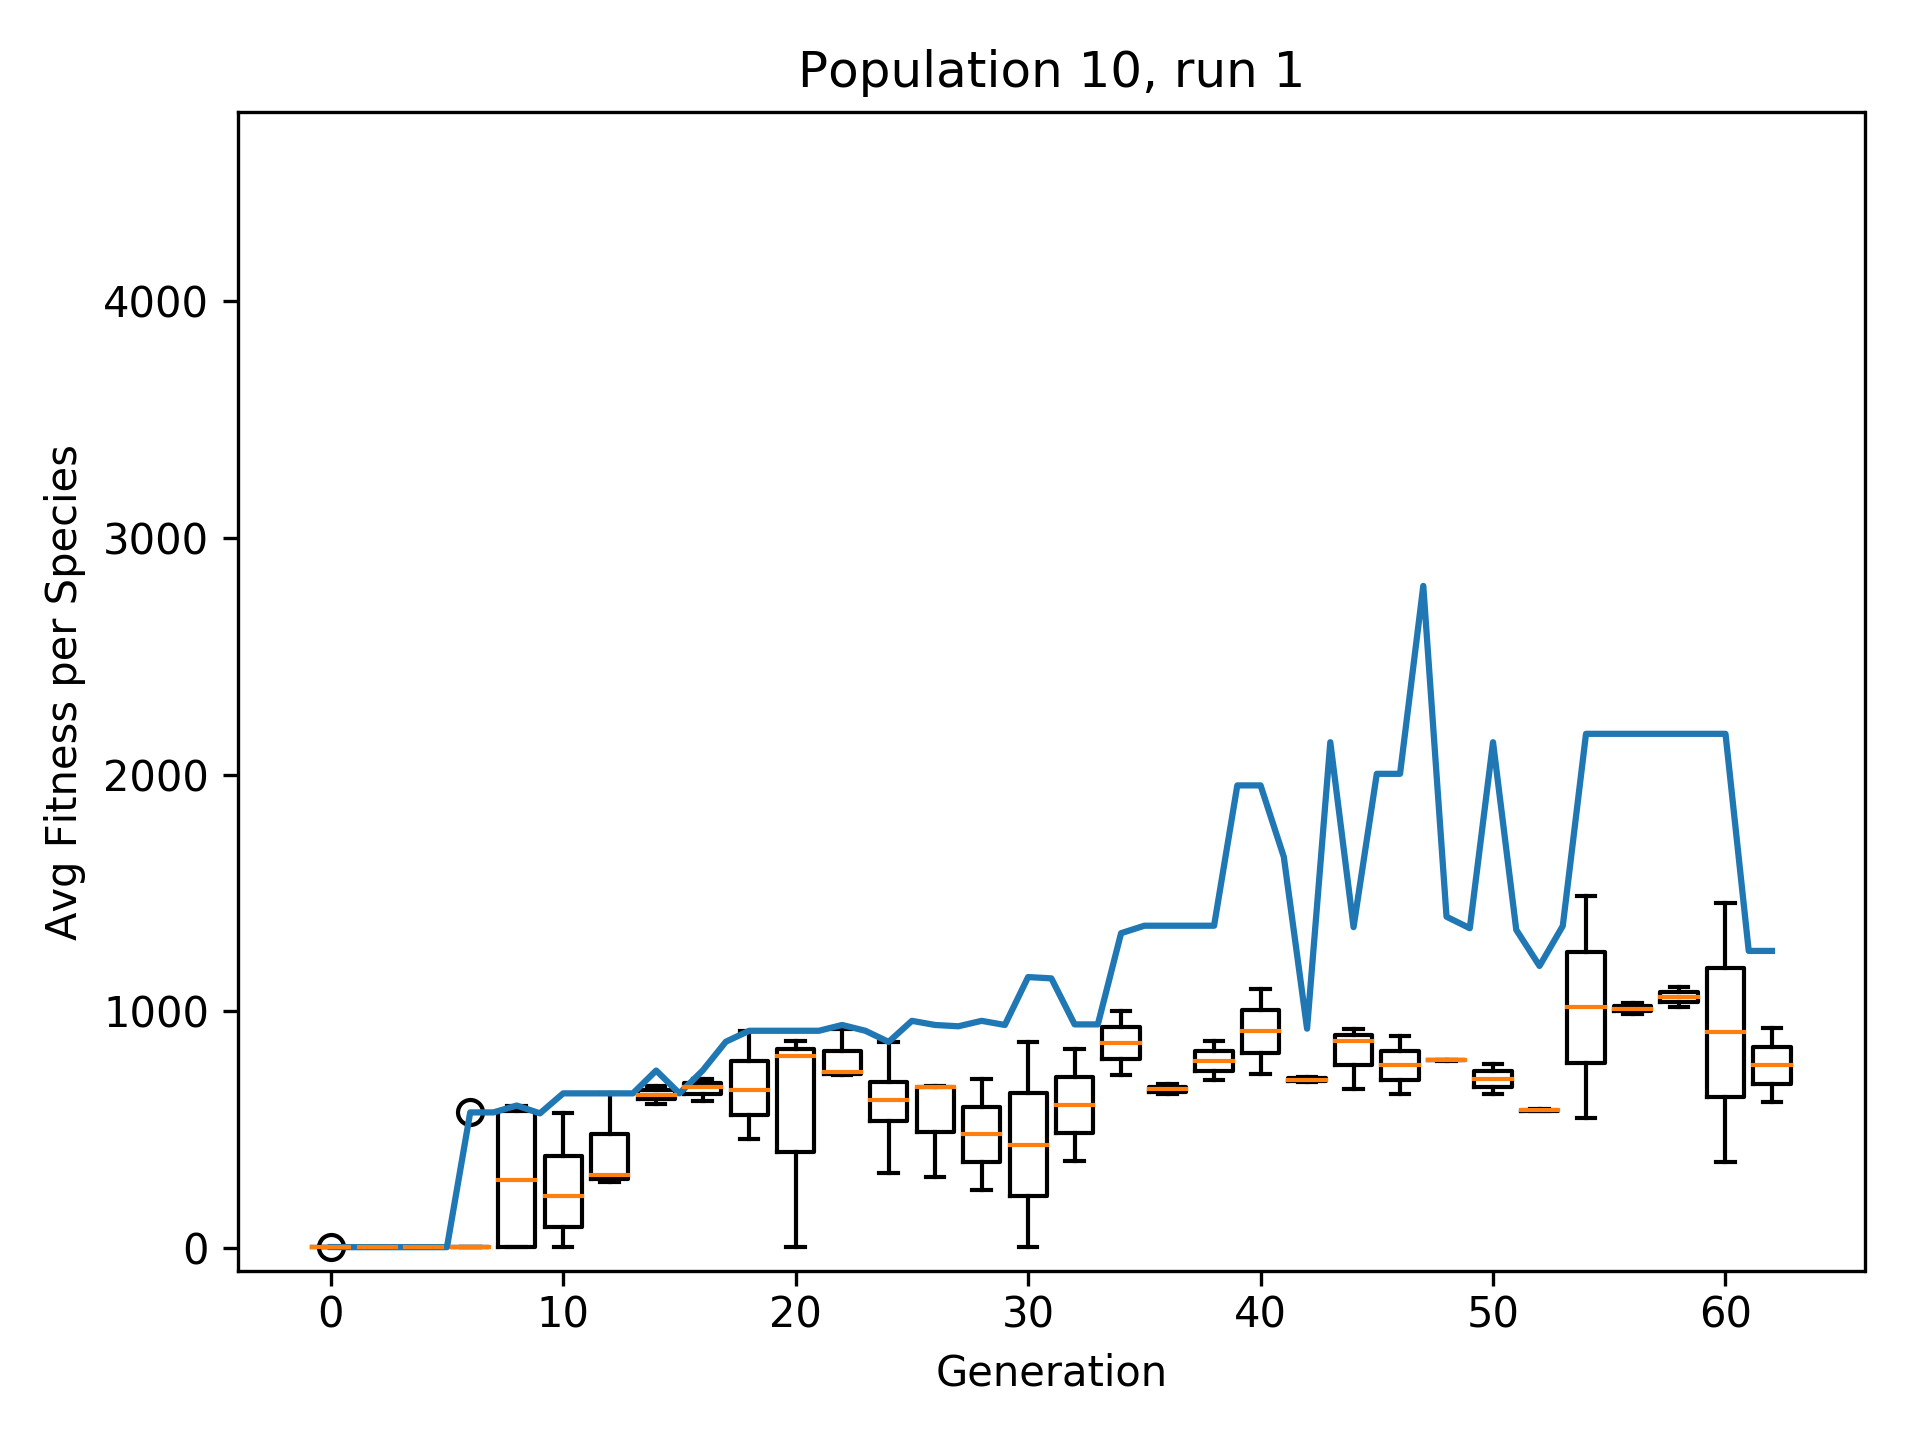
\includegraphics[width=1\textwidth]{graphics/mario/pop10_run1} % first figure itself
%				\end{minipage}\hfill
%				\begin{minipage}{0.33\textwidth}
%					\centering
%					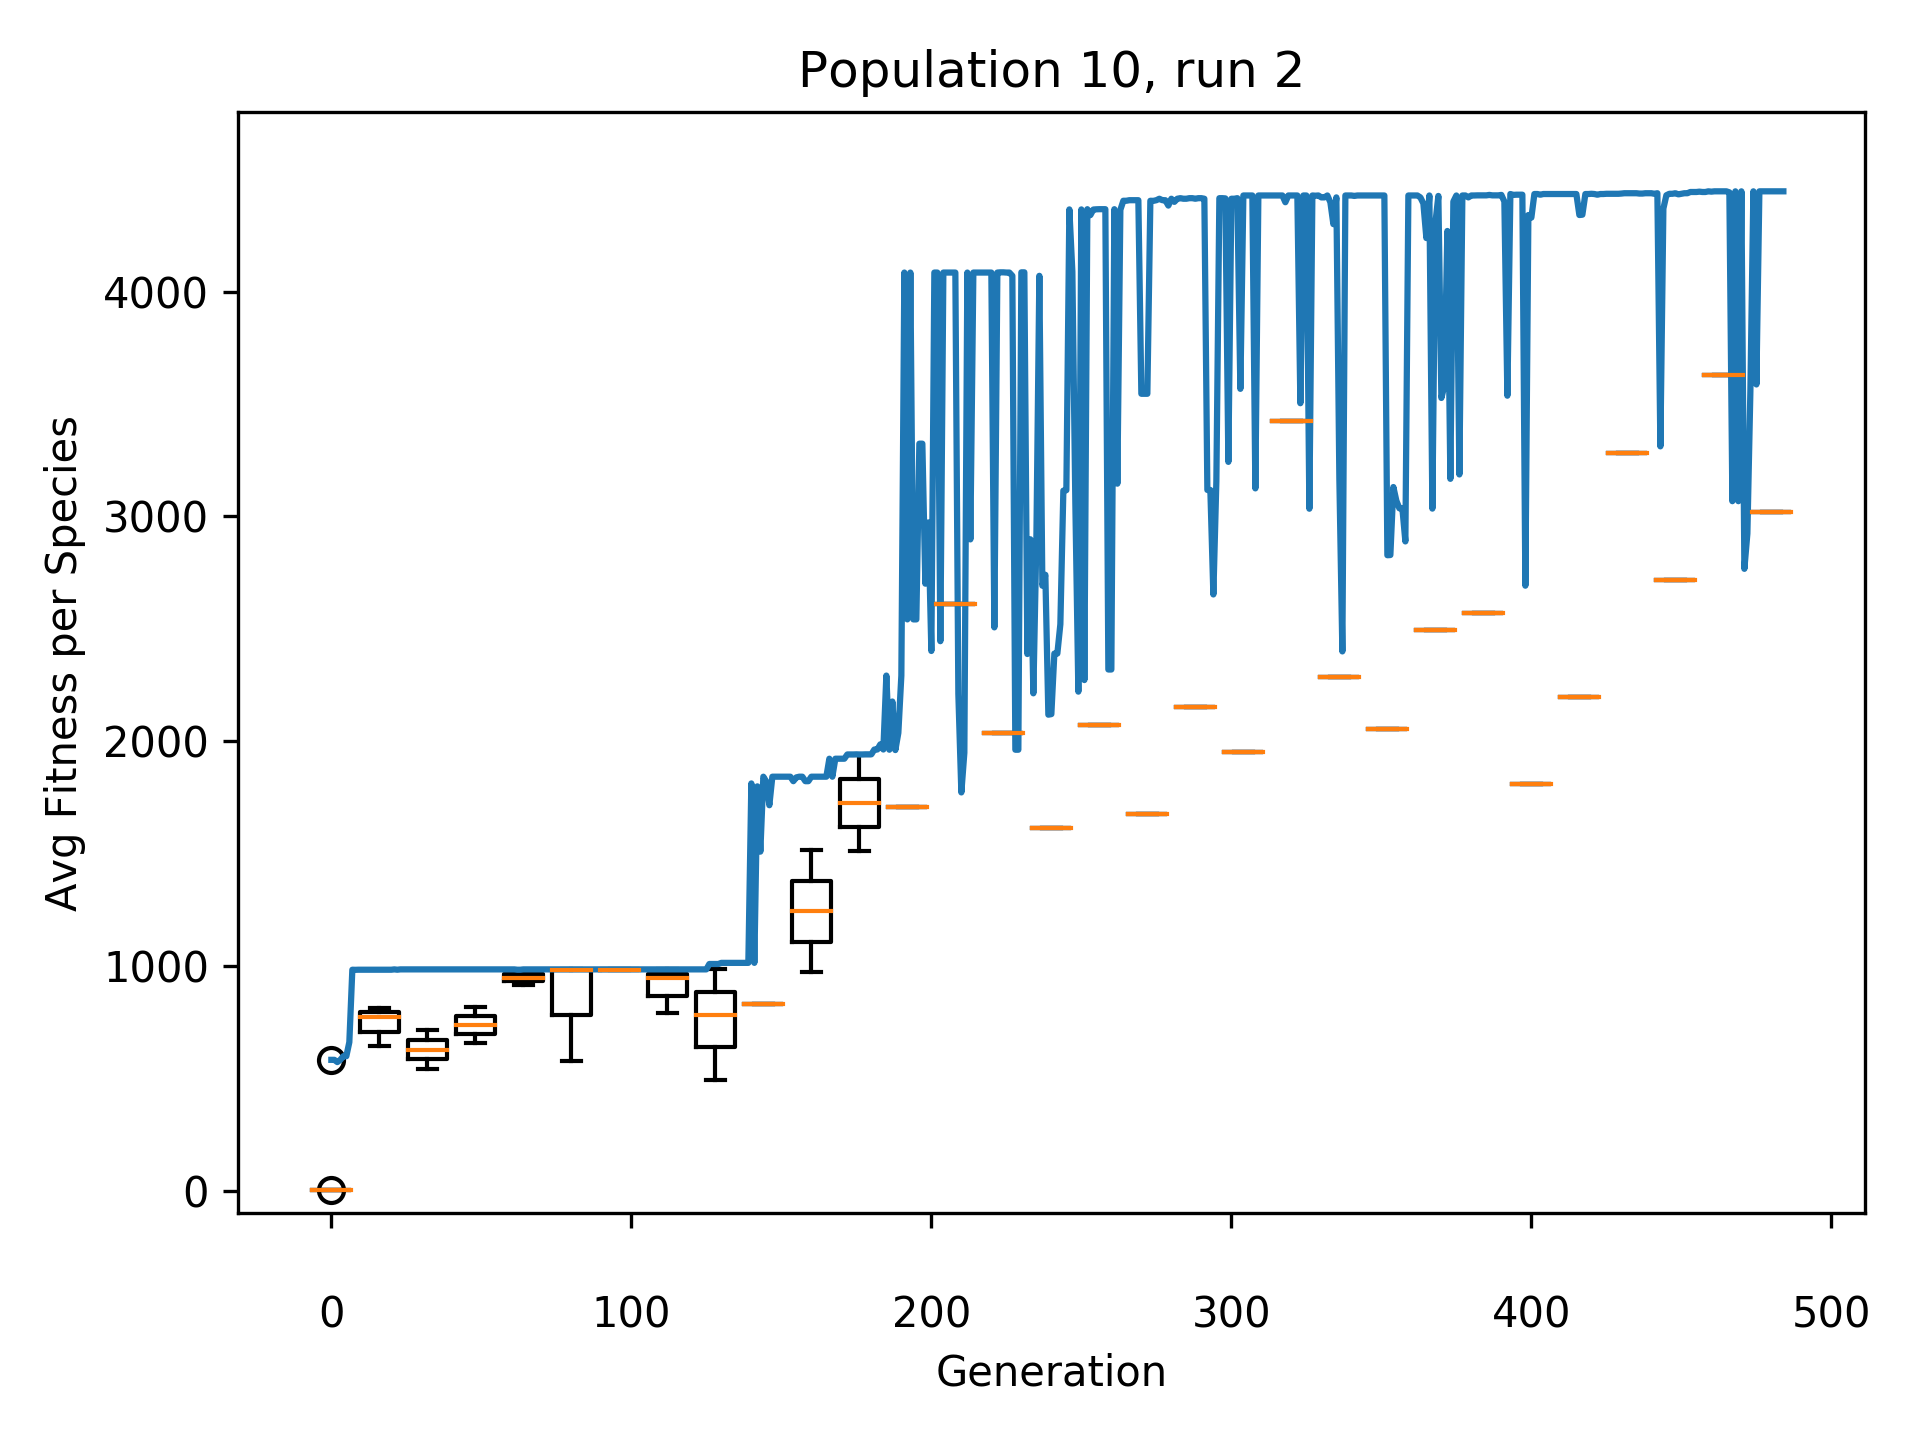
\includegraphics[width=1\textwidth]{graphics/mario/pop10_run2} % second figure itself
%				\end{minipage}
%				\begin{minipage}{0.33\textwidth}
%					\centering
%					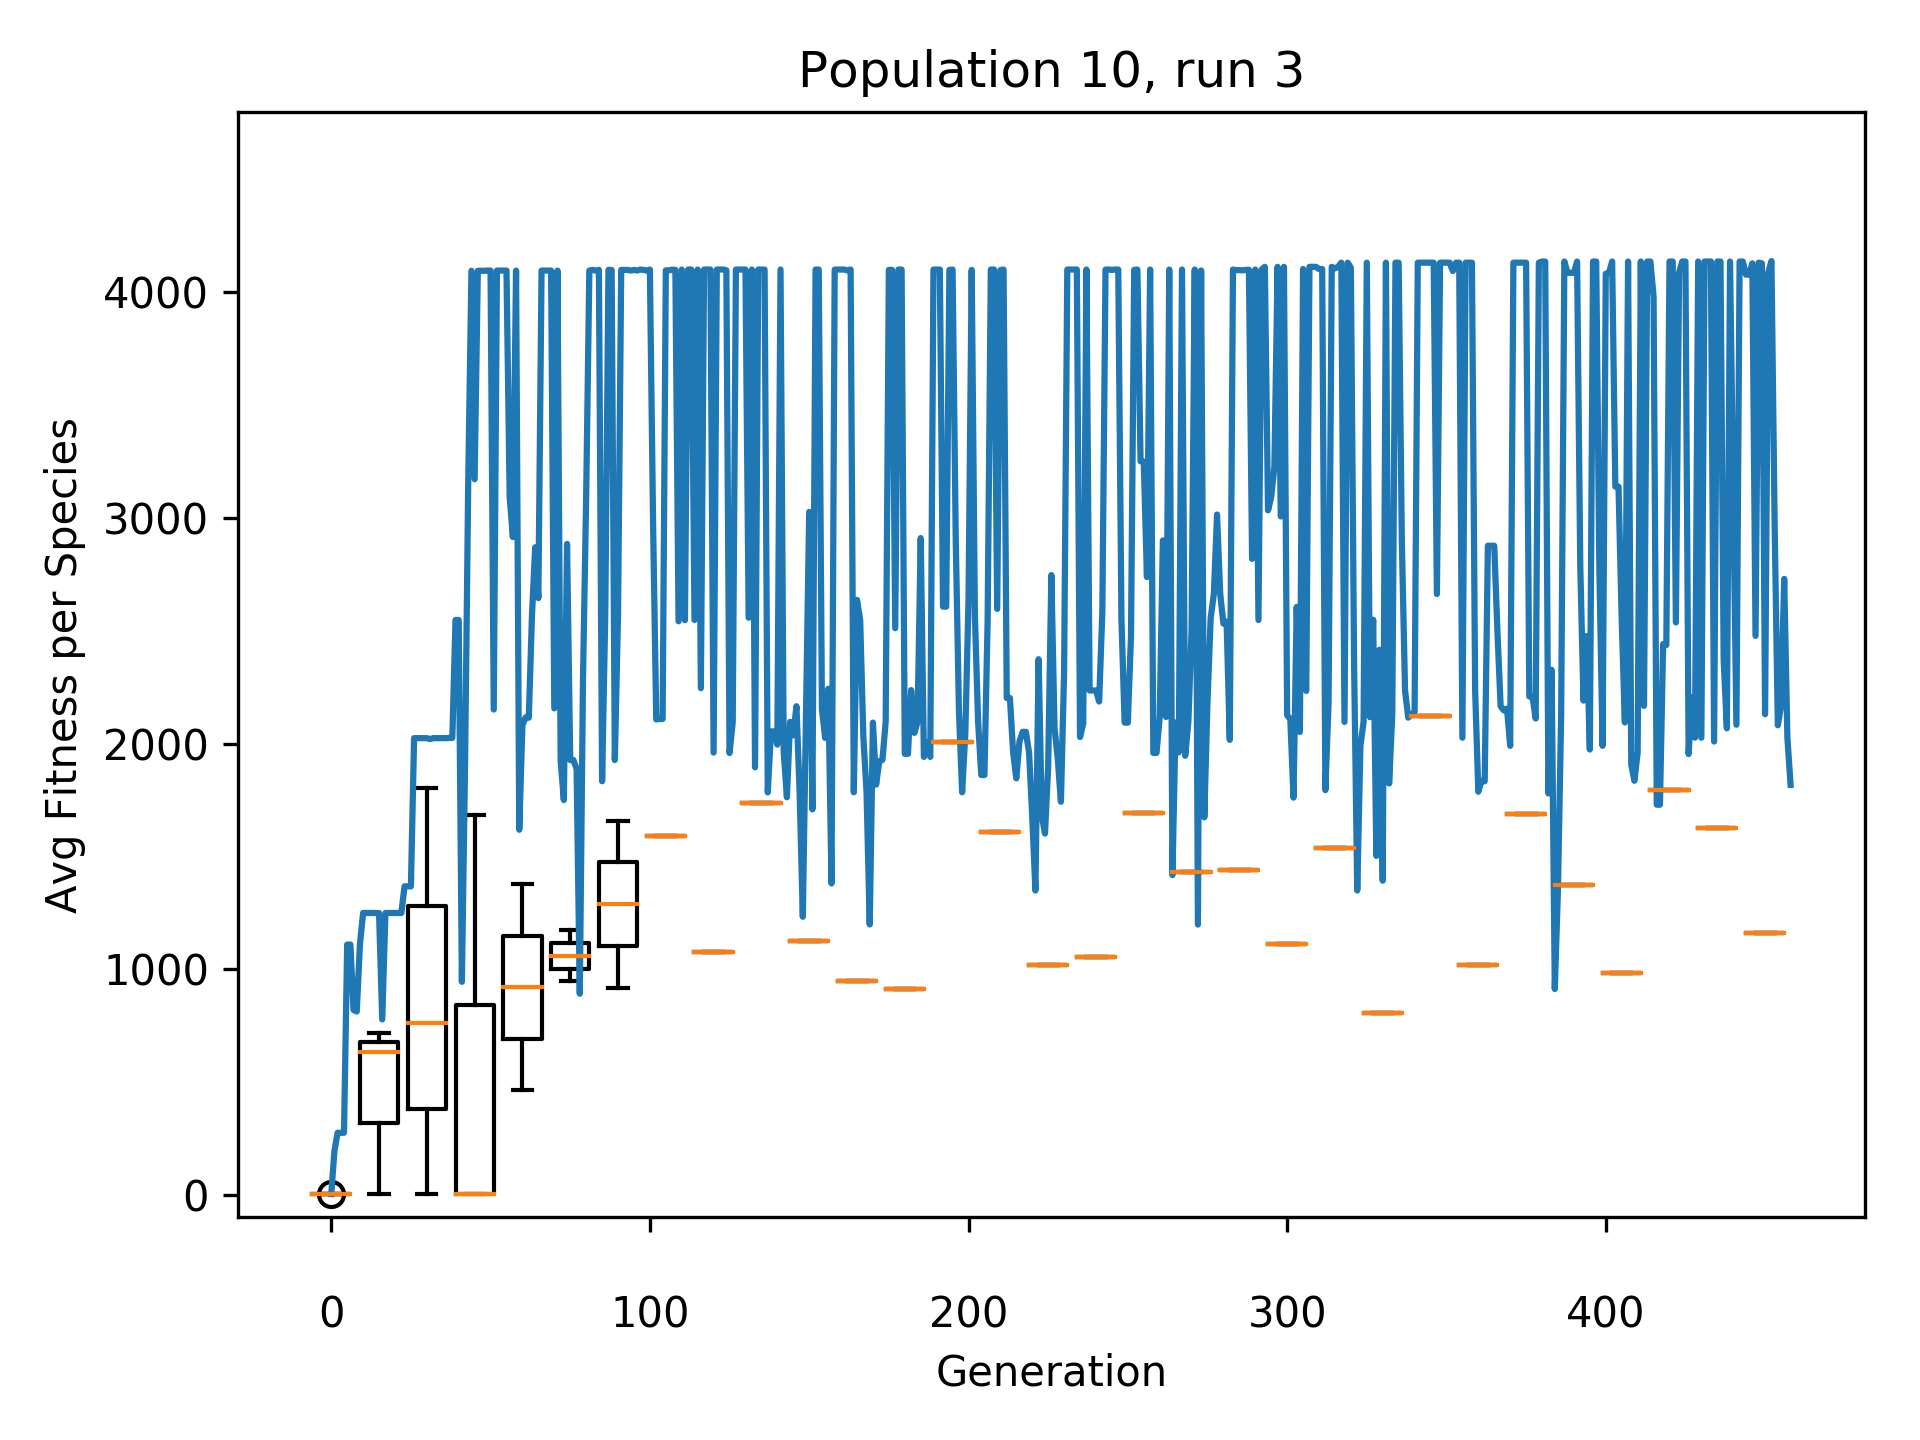
\includegraphics[width=1\textwidth]{graphics/mario/pop10_run3} % second figure itself
%				\end{minipage}
%				\caption{MarI/O Population 10}
%				\label{fig:mario10}
%			\end{figure}
			As it is visible in Figure \ref{fig:mario10} the vertical axis shows the fitness score average of the genomes within a species. The horizontal axis portrays the generations containing the species. Each generation contains up to 10 populations which is divided into species and genomes within species. This species devision was made based on the NEAT algorithm described in section \ref{sec:related:neat}. The best run of the genomes grouped by each generation is marked with a blue line. Therefore the blue line indicates the best overall run within a generation. Since the boxplot portrays the species's avarage score of each generation and the the blue line shows the best run per genome (population), the boxplot and the blue line rarely meet. Still the average population score is closer to the best run than in the next two population variants (see later in this section population 50 \ref{par:mario50} and population 250 \ref{par:mario250}). This can be calculated by taking the median of the species fitnesses and substracting that number from the best run of the genomes:
			$average\_distance = \frac{\sum\nolimits_{g_i \in generations} max(g_i.genomes) - median(g_i.species)}{|generations|}\approx1107$ whereas $g_i.genomes$ and $g_i.species$ are lists of the respective fitnesses. \\
			In the three runs on average $334.\overline{6}$ generations were created which results in a skipping of generations inside the graphics of around $11.1\overline{5}$ generations averagely between two displayed generations. Unfortunately the first run crashed after generation 60. Still, because of the long runtime of the simulation the run was kept. However, indicated by plot run 2 and 3, the population growth started after this generation. As it can be seen in the 3rd run of the figure \ref{fig:mario10}, sometimes runs over 3000 fitness score could be achieved even after the 30th generation. In run 2 the average fitness of the species tend to rise, however more and longer runs would be needed to test this hypothesis.\\
			In each generations there are up to 10 populations. \todo{(up to because of neat implementation check neat implementation}
			In the first generation (Gen 0) no mating was done, so in the first generation there where 10 species spawned with one genome each. In the 10th Generation on average only $4.\overline{3}$ species where left. After generation 50 maximum 3 species where left in all runs and after generation 190 in run 2 and after generation 91 in run 3, respectively, only 1 species was left for mating. The mating results into the corssover of species.\\
			All runs except plot run 1 reached the goal (the end of the level) multiple times which can be seen by the fitnesscore being over 4000. However plot run 3 reached the goal the earliest with runs over 4096 starting from generation 44. Still there was the most overall regress made in plot run 3. This can be calculated by adding the differences between the best runs of each generation if the difference was negative: $average\_regress = \frac{\sum\nolimits_{g_i \in generations} min(max(g_i.genomes) - max(g_{i-1}.genomes), 0)}{|generations|}\approx-348$ again whereas $g_i.genomes$ is a list of the fitnesses of each genome inside the generation. The regress of plot-run 1 was $-88.27$ approximately and of plot-run 2 was around $-109.98$.\\
			In plot run 1 the $average\_fitness\_increase =  \frac{\sum\nolimits_{g_i \in generations} max(g_i.genomes) - max(g_{i-1}.genomes)}{|generations|}\approx19.87$ was the biggest of the three runs since run 1 ended early and run 3 had many drawbacks. The average fitness increase of run 2 was around $7.97$ and of run 3 was only $3.95$ approximately. Since it is only slightly possible to extend the maximum score above the score of 4000 and run 1 has never reached this ranking, run 1 pointed out to have the best score increase per round. Every successful round, whereas Mario reached the goal will only minimize the fitness increase when averaged with the generation count. In another words, for an infinitely large amount of generations the $average\_fitness\_increase$ is expected to converge to $0$ since the game has and end-state in contrast to the game Flappy Bird, as it can be seen in section \ref{sec:analysis:flappy}. In mathematical terms: $\lim\limits_{n \to \infty} average\_fitness\_increase(n) = 0$, whereas the $average\_fitness\_increase(n)$ is defined as the average fitness increase of a set of n generations.
			
			\begin{enumerate}
				\item there are up to 10 populations in each generation (up to because of neat implementation \todo{check neat implementation})
				\item Differences similarities between runs
			\end{enumerate}
		
		\paragraph{Population 50 / Generation 100}
			\label{par:mario50}
			\begin{figure}[h]
				\centering
				\begin{minipage}{0.33\textwidth}
					\centering
					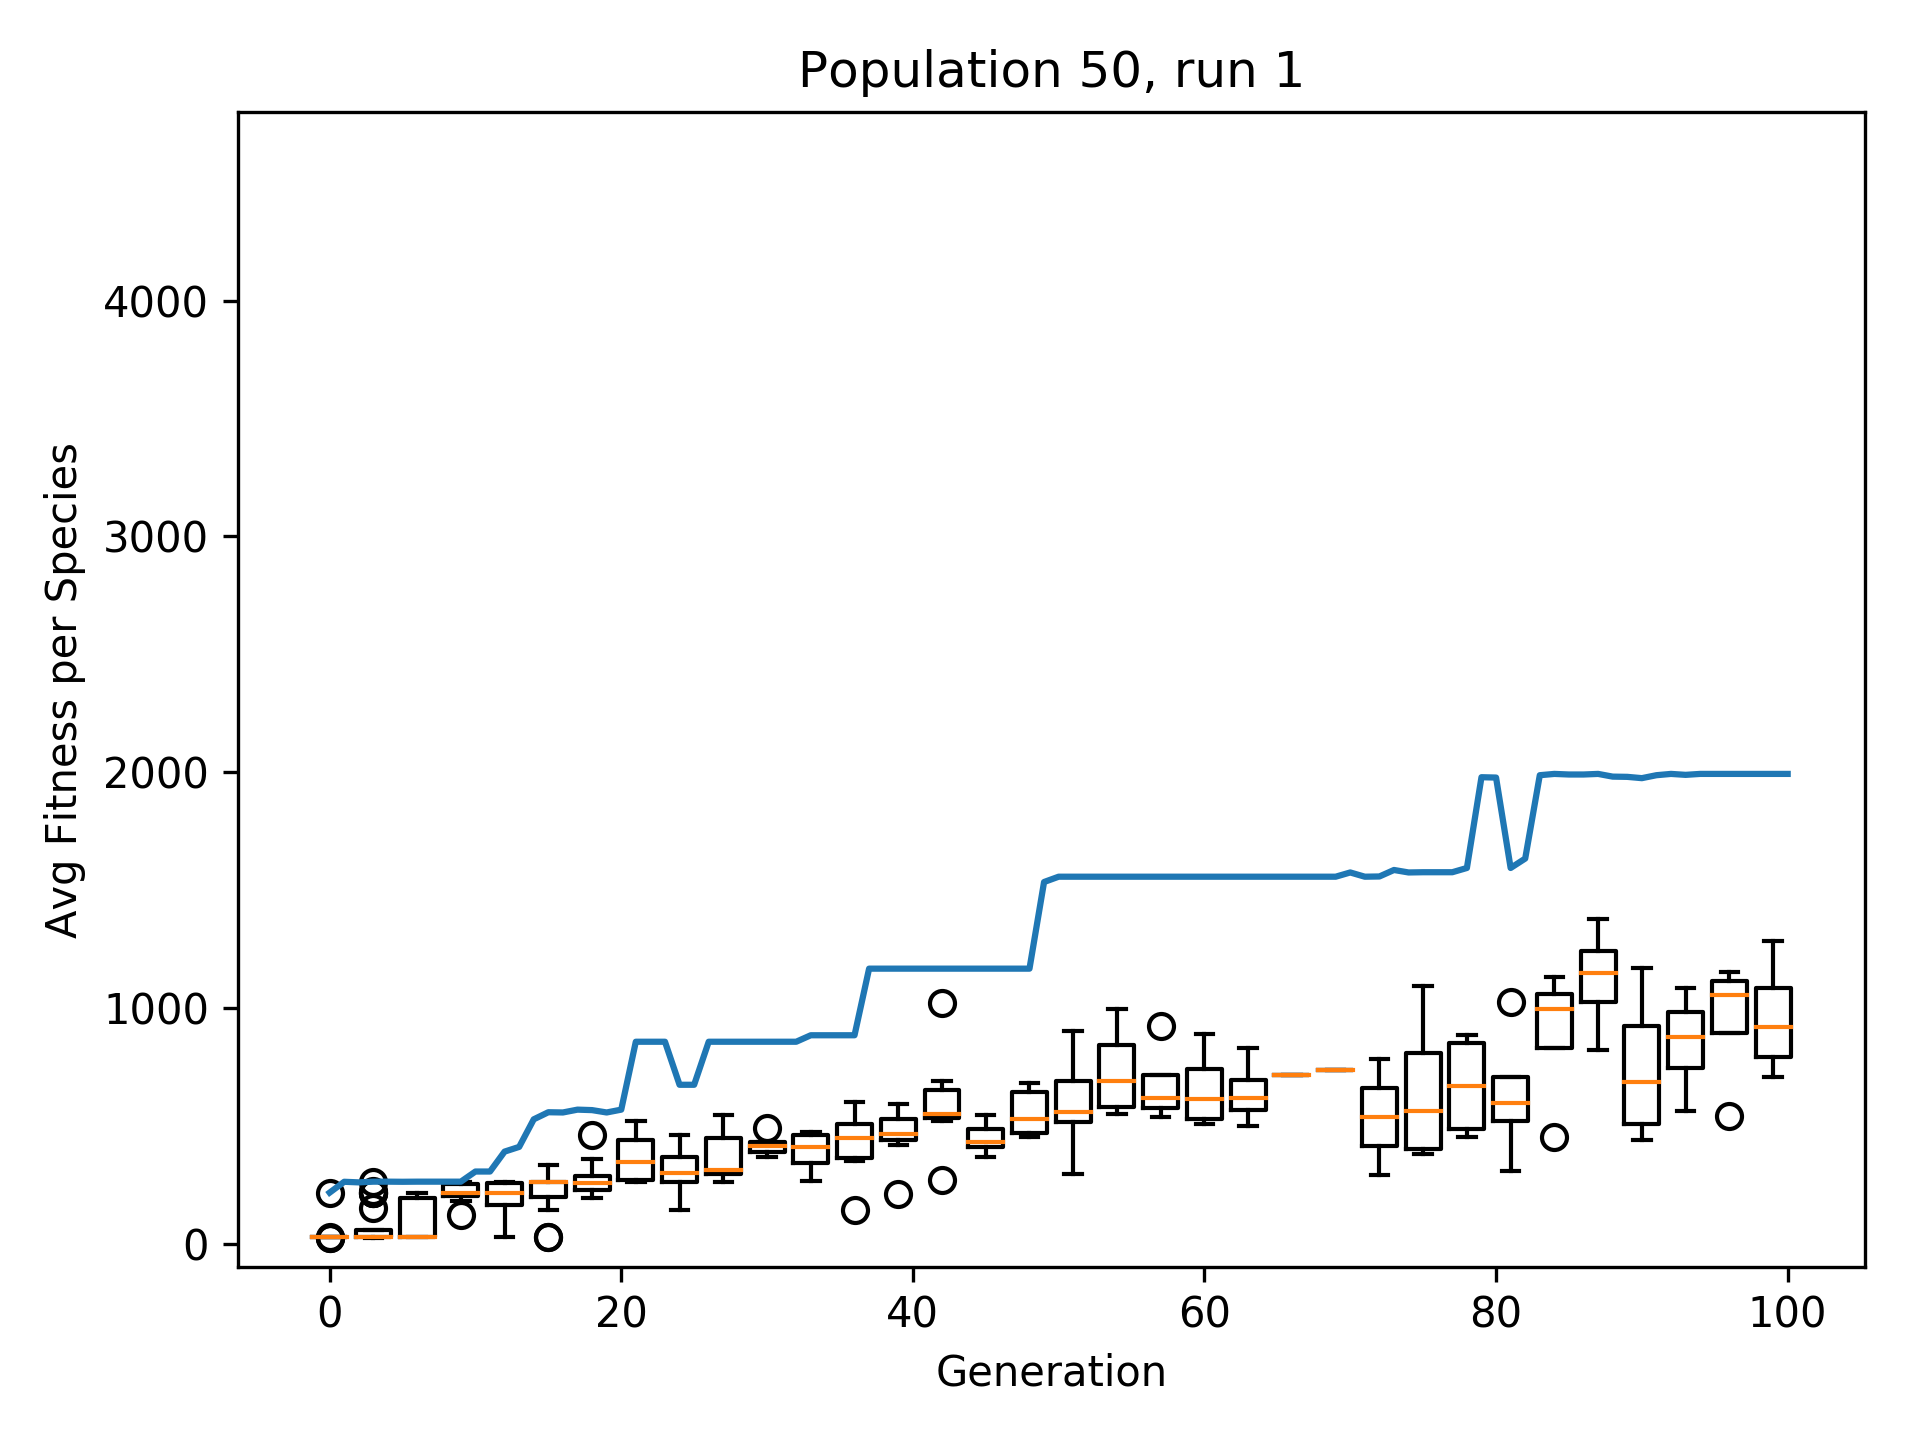
\includegraphics[width=1\textwidth]{graphics/mario/pop50_run1} % first figure itself
				\end{minipage}\hfill
				\begin{minipage}{0.33\textwidth}
					\centering
					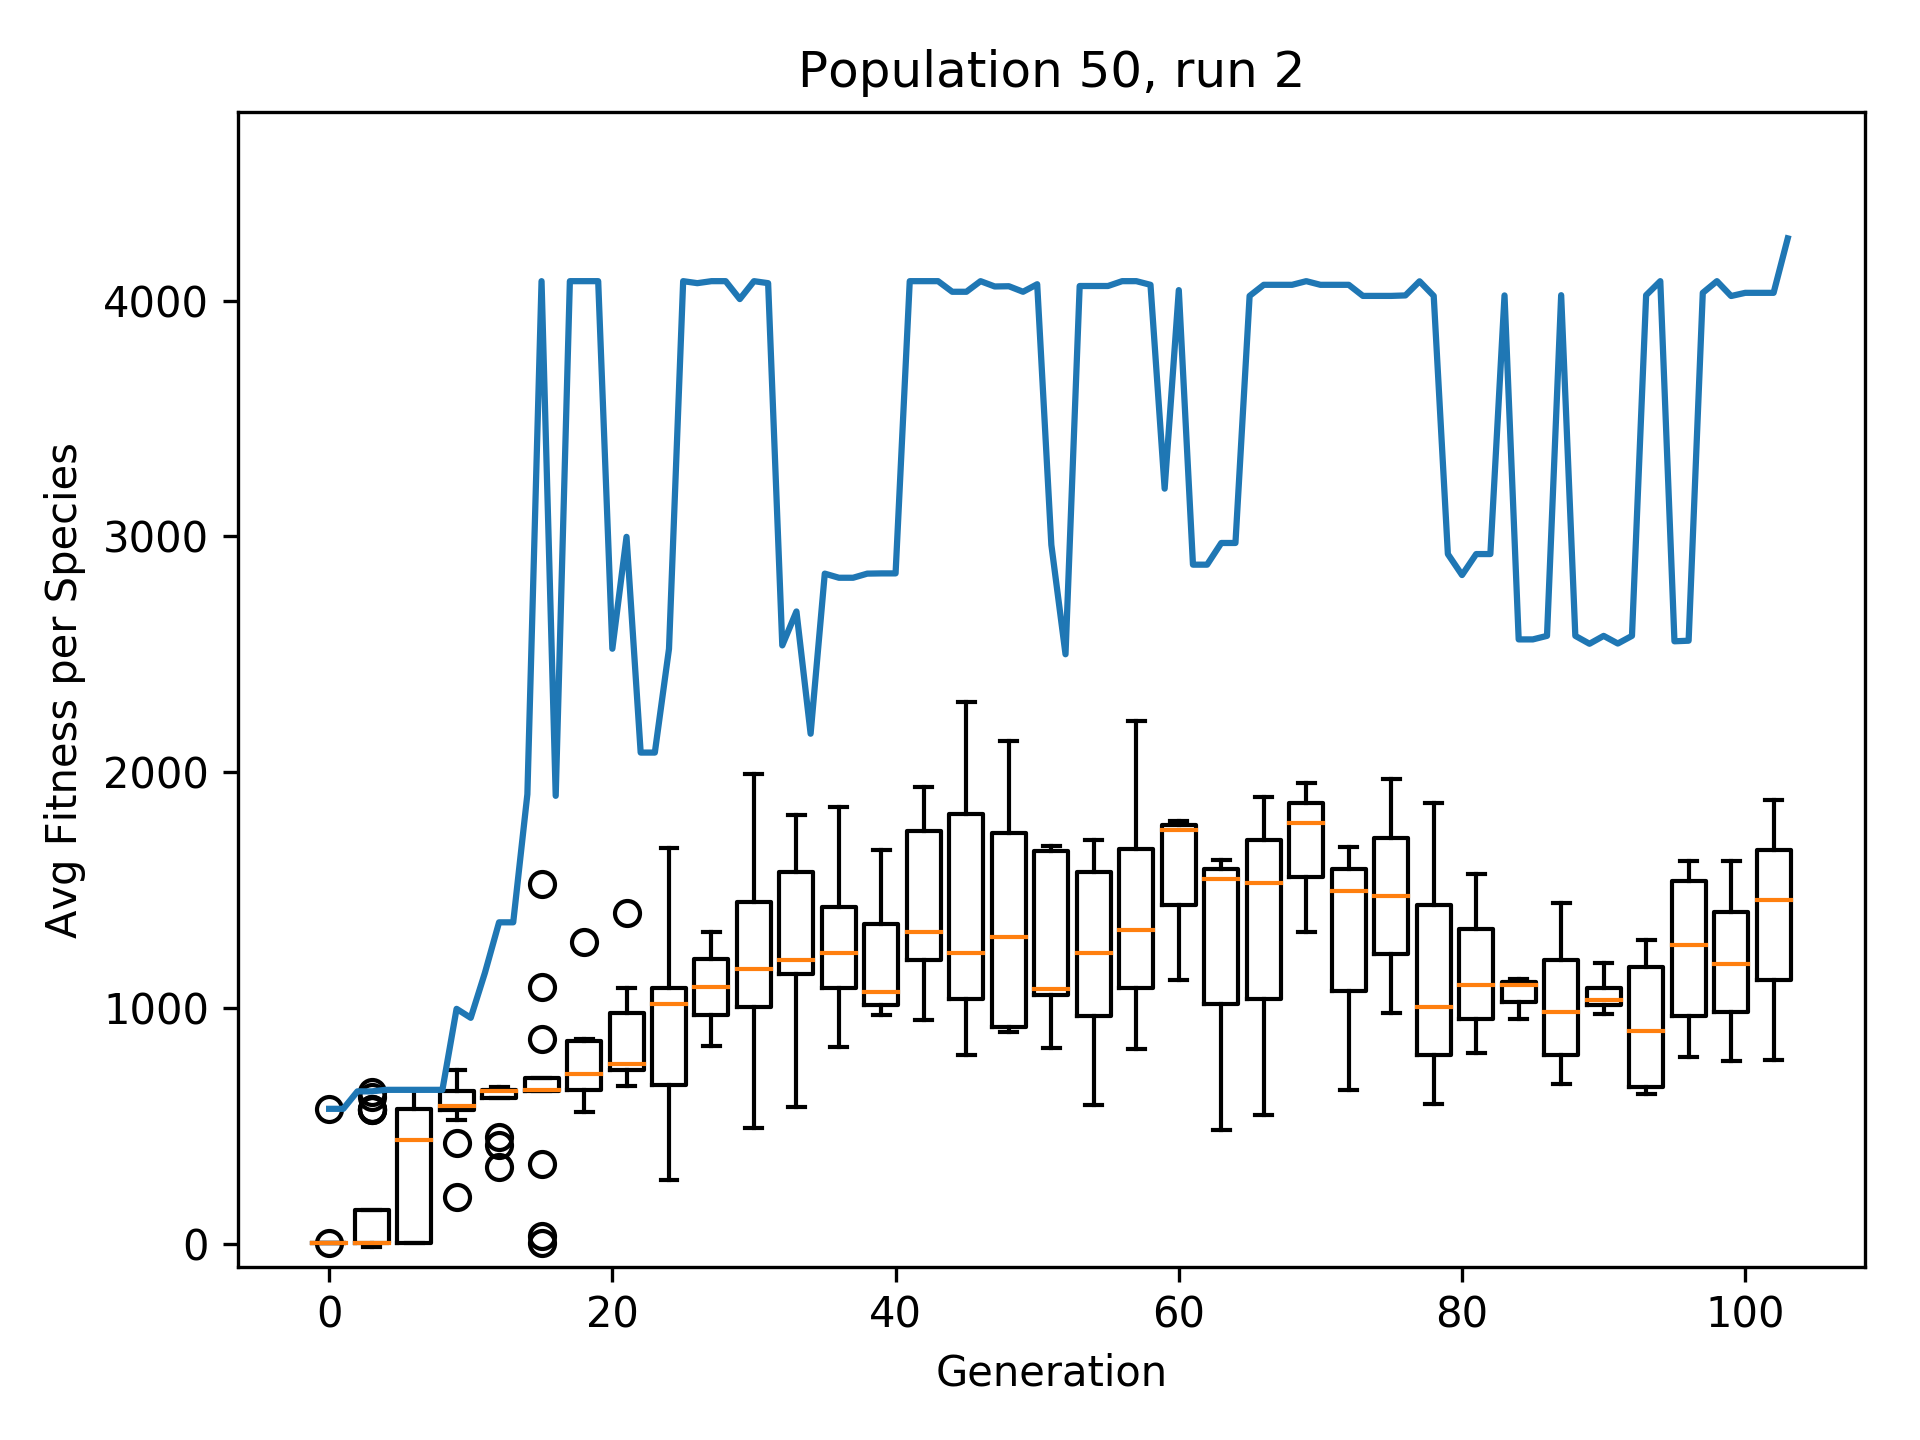
\includegraphics[width=1\textwidth]{graphics/mario/pop50_run2} % second figure itself
				\end{minipage}
				\begin{minipage}{0.33\textwidth}
					\centering
					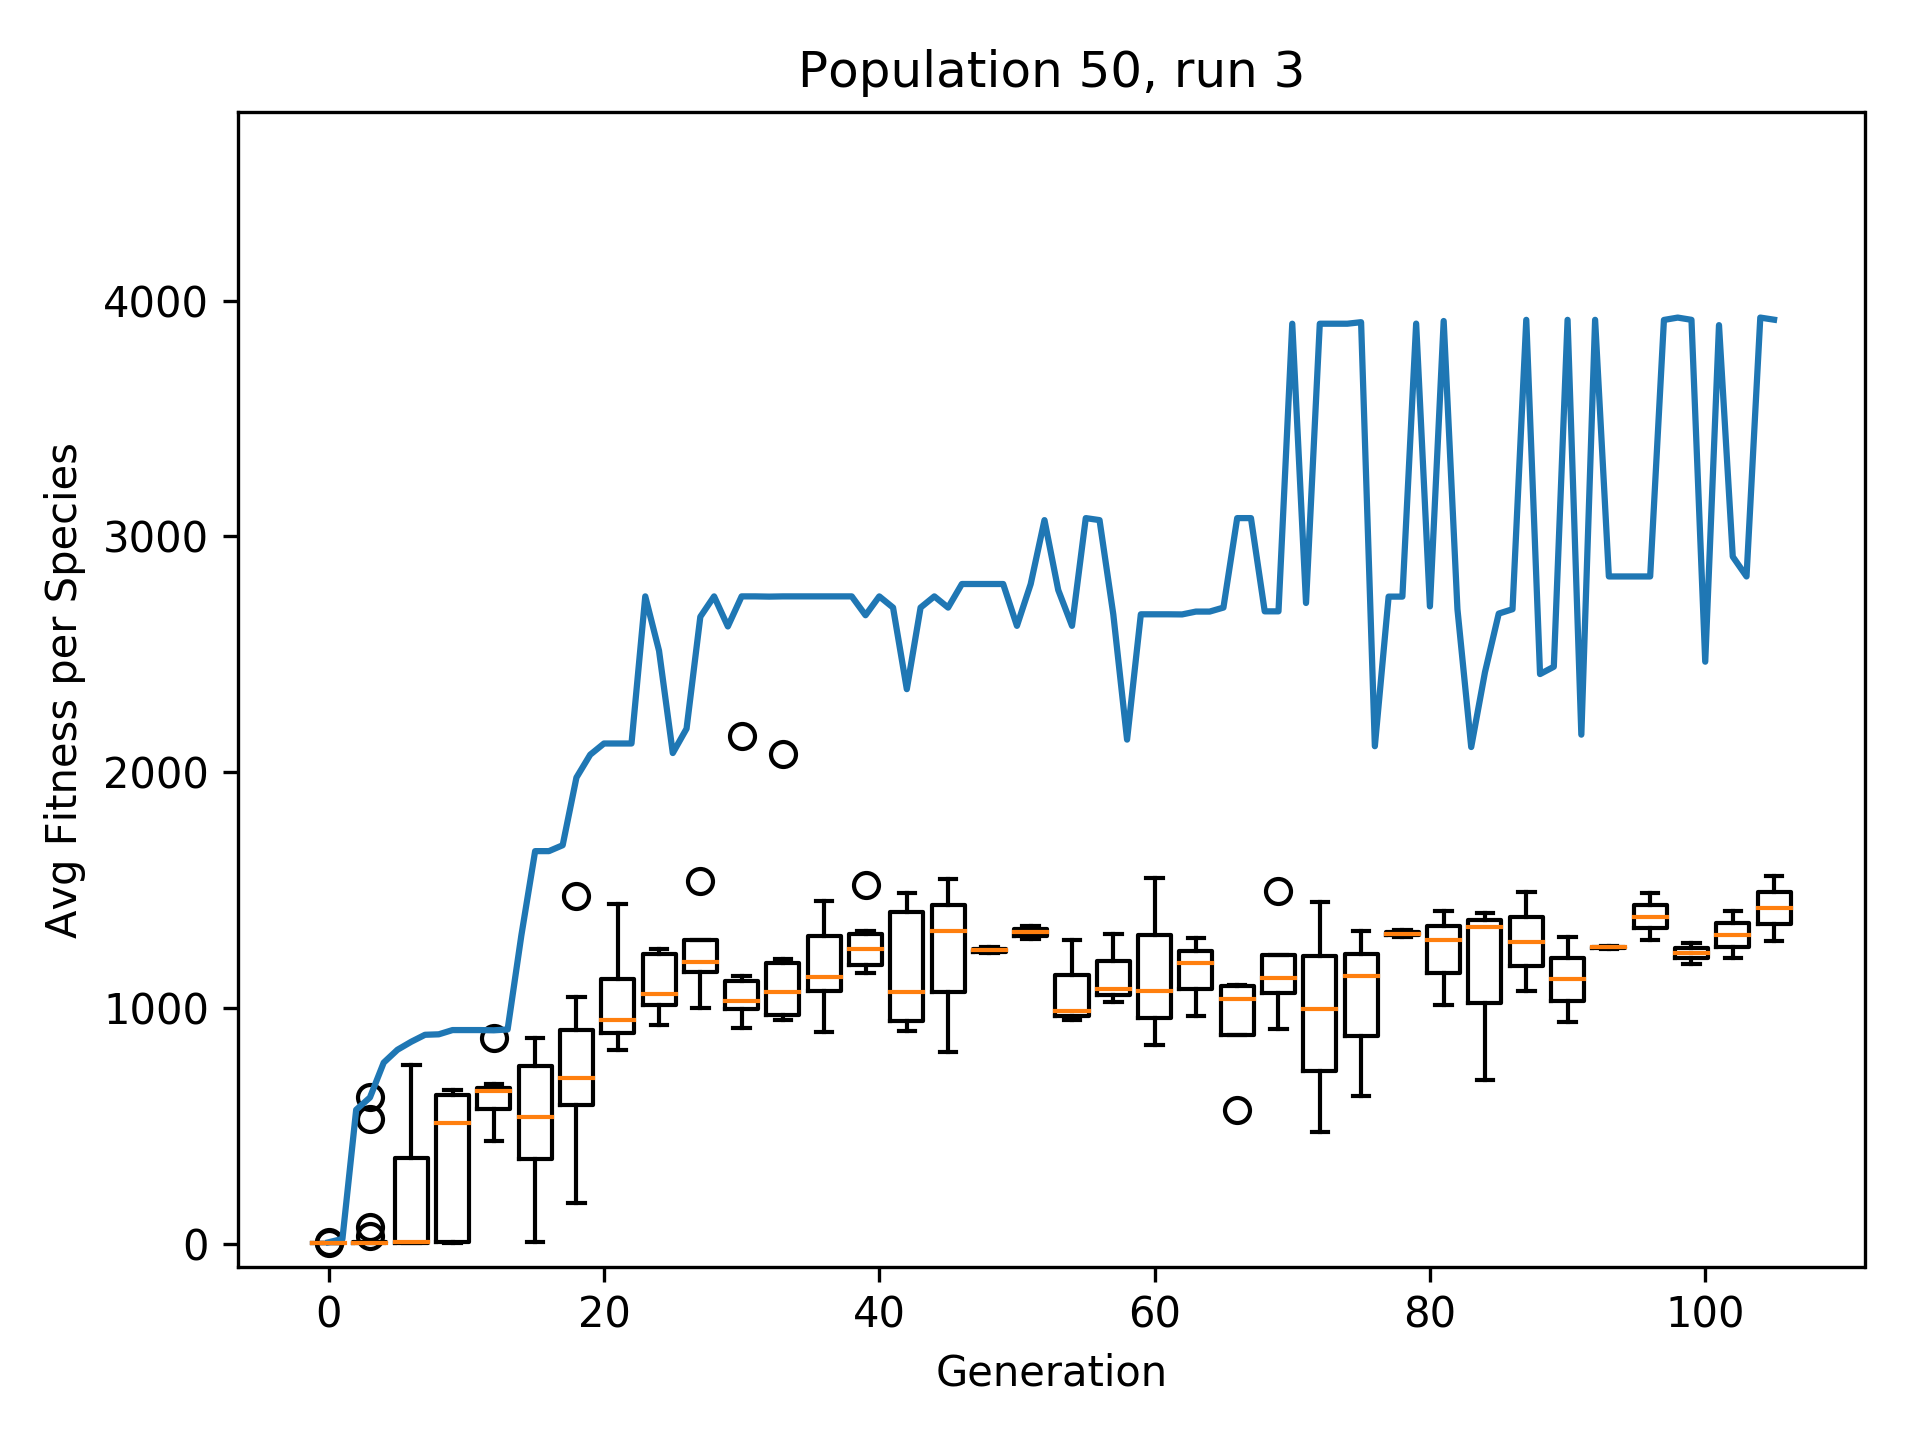
\includegraphics[width=1\textwidth]{graphics/mario/pop50_run3} % second figure itself
				\end{minipage}
				\caption{MarI/O Population 50}
				\label{fig:mario50}
			\end{figure}
			In this setup the population count is up to 50, again distributed into species and genomes within species according to the MarI/O NEAT implementation. The $average\_distance$  between the median of the species of each generation to the best genome run of this generation is bigger than that of the simulation with it's initial population size of 10 but it is smaller than in the last case. The $average\_distance$ was calculated as described in the previous simulation (population 10 \ref{par:mario10}) and the value is approximately $1406$.\\
			In this simulations the runs where executed until there where over 100 generations (101 generations in run 1, 104 in run 2 and 106 in run 3). This results in an average skipping of 3.456 generations between the display of two generations.\\
			In generation 0 there where 50 species spawned, again, with one genome each. In the 10th generation there where 15 species left on average. At the end of generation 100 on average $3.\overline{3}$ species where left from the initial 50 generations.\\
			Interestingly the plot run 1 couldn't learn to reach the goal. From this data it is not trivial to predict if the breakthrough would have started within the next 50 generations or if this run would have stayed low in it's fitness score, since there are no clear patterns to find in the graphical representation of these runs. In order to answer on this question more profoundly, further and longer runs have to be made and the big jumps between the fitness scores of each neighbour generation would have to be analysed.\\
			Plot run 2 and 3 had more luck in reaching the end, however run 3 had more stability in it's high score results between generations. Still after generation 70 plot run 3 also shows stronger differences between it's generation's heigh scores. Nevertheless, plot-run 2 reached the goal the earliest. The first time run 2 acheived a fitness-score over 4000 was in generation 15 (it reached a score of $4082.5$), whereas plot-run 3 reached a maximum score of $3928$ in generation 98. Still run 3 reached to goal with a score of $3902$ the first time in generation 70. The 3rd plot-run has the highest $average\_fitness\_increase\approx36.92$ of the three runs. Plot-run 1 has an $average\_fitness\_increase$ of $17.58$ approximately and plot-run 2 of $35.5$ precisely.\\
		
		
		\paragraph{Population 250 / Generation 30}
			\label{par:mario250}
			\begin{figure}[h]
				\centering
				\begin{minipage}{0.33\textwidth}
					\centering
					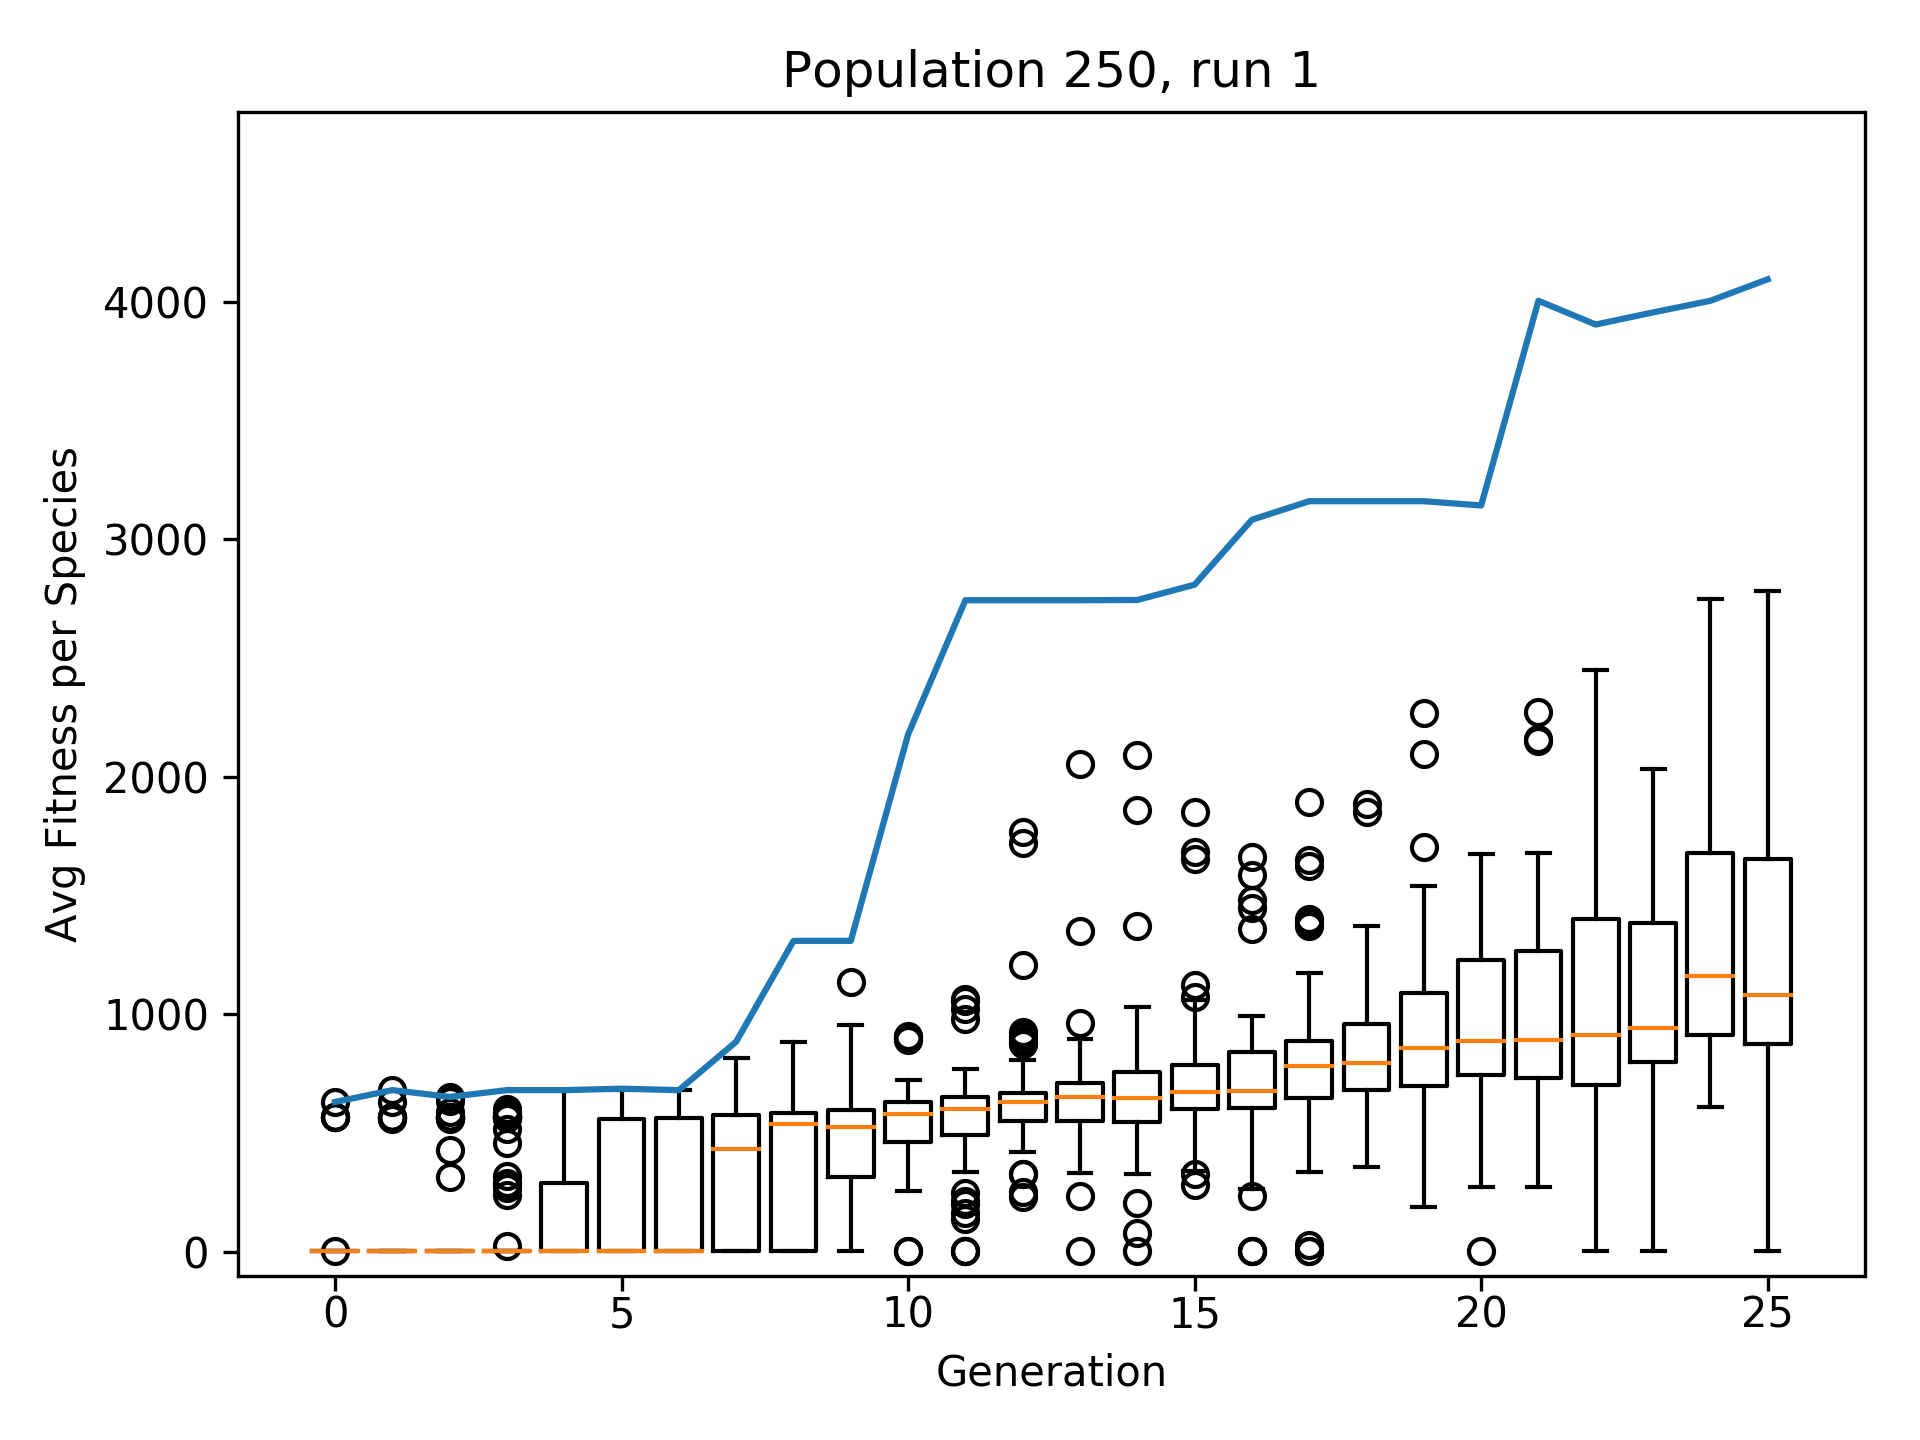
\includegraphics[width=1\textwidth]{graphics/mario/pop250_run1} % first figure itself
				\end{minipage}\hfill
				\begin{minipage}{0.33\textwidth}
					\centering
					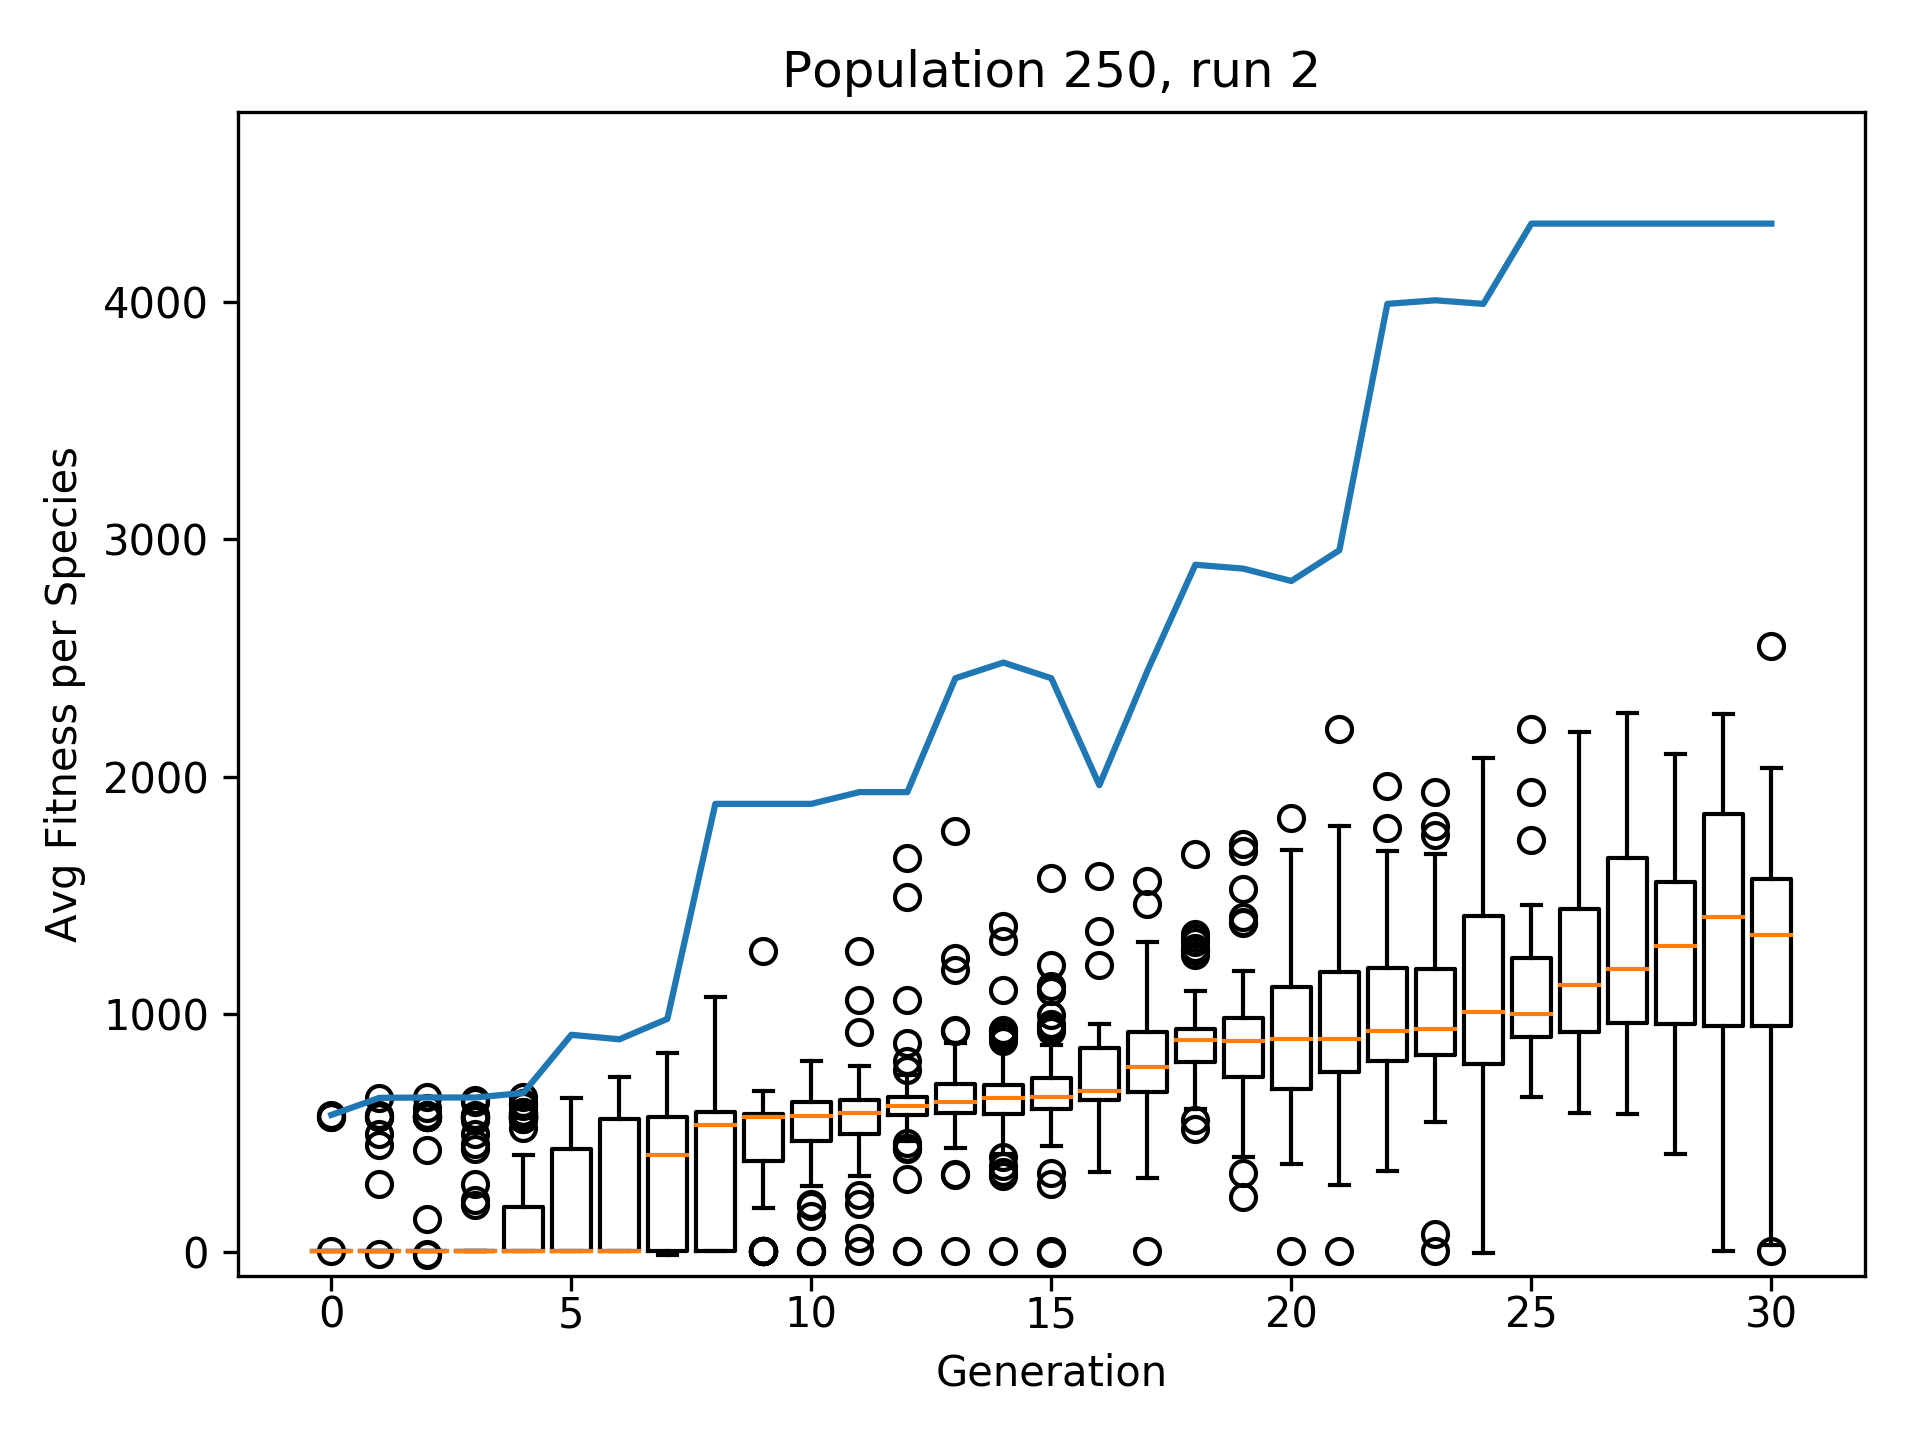
\includegraphics[width=1\textwidth]{graphics/mario/pop250_run2} % second figure itself
				\end{minipage}
				\begin{minipage}{0.33\textwidth}
					\centering
					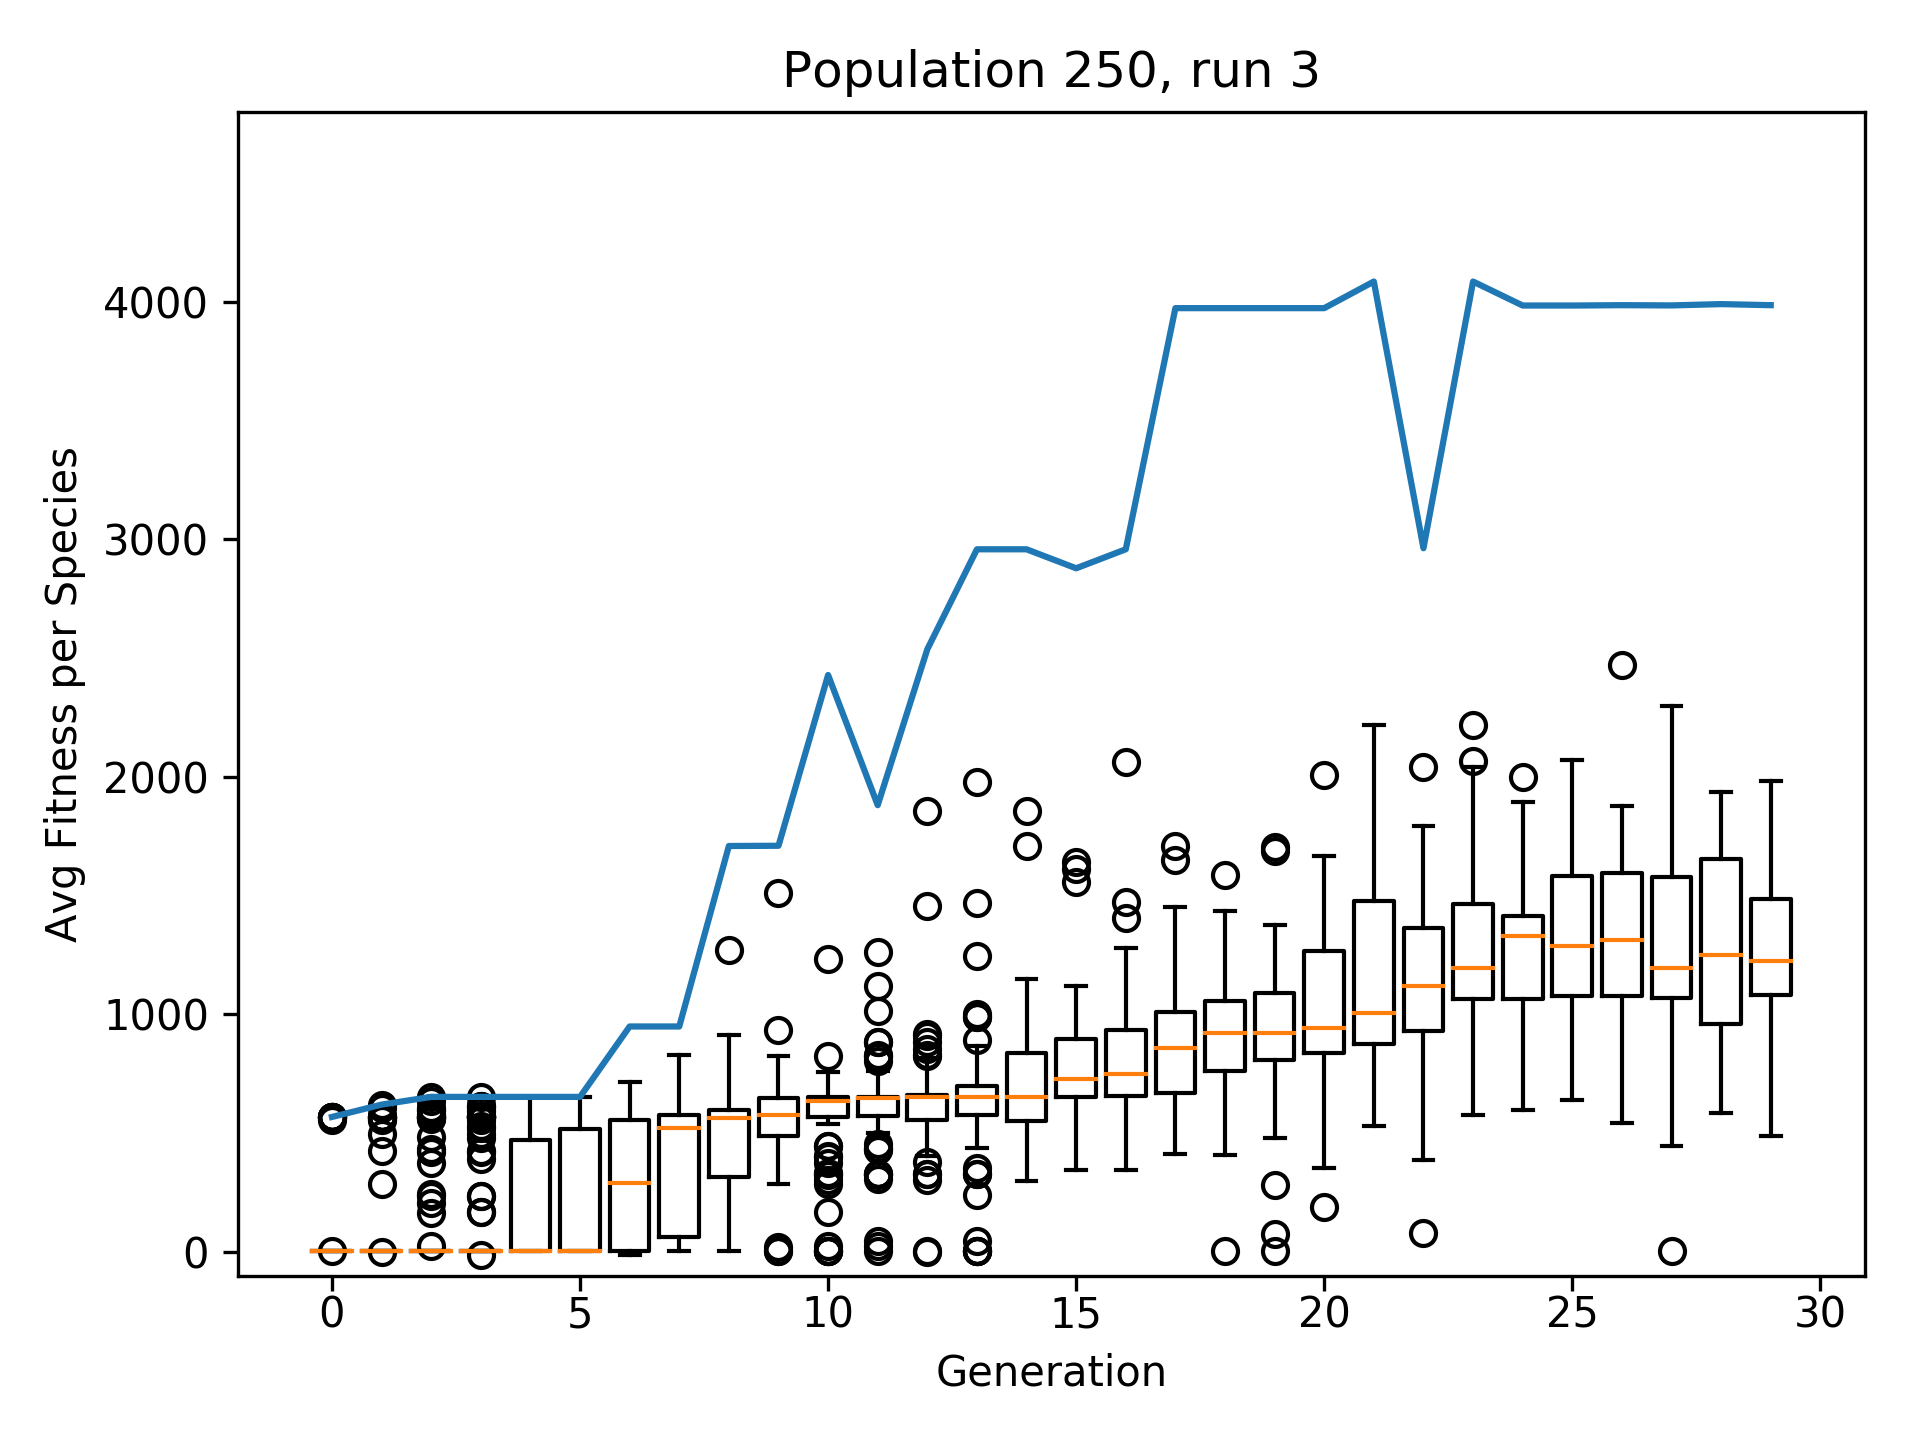
\includegraphics[width=1\textwidth]{graphics/mario/pop250_run3} % second figure itself
				\end{minipage}
				\caption{MarI/O Population 250}
				\label{fig:mario250}
			\end{figure}
			In figure \ref{fig:mario250} the population size is up to 250 in generation 0. In the first generation (Gen 0) 250 species are born with one genome each. The $average\_distance$ for this plot-runs is the biggest with approximately $1827$ when compared to the plot-runs with an initial population size of 10 and 50. In this plots no generations had to be skipped in order to portray a descriptive graph since the maximum generation count is 30 in run 2 (25 generations in run 1 and 29 generations in run 3).\\
			Already in the 6th generation, on average only 94.8 species where left. At the end of generation 25 there where 31 species left on average. \\
			Compared to the other two population classes there are at least 7 times more species left at the end of the simulations which results in longer whiskers of the boxplot.The wiskers even contains bad starts with fitness-scores lower than 100 in plot-run 1 and 2. Interestingly the best runs are always exceptions after generation 6 (in plot-run 1 and 2 even earlier). \\
			Further it is to mention that the plots are rather uniform compared to the plots of population 10 and 50. Therefore the $average\_fitness\_increase$ has similar values with a low variance which are $133.25$ for generation 1, around $121.08$ for generation 2 and $113.95$ for generation 3. The $average\_regress$ is the lowest in run 1 with $-5.87$ approximately. This is because the maximum value of the succeeding generation is smaller then the previous generation in only 4 cases. The other two plot-runs have an $average\_regress$ of approximately $-19.97$ in run 2 and $-61.92$ in run 3. All of the runs reached the end of the level even thought run 3 reached the end at generation 17, whereas plot-run 1 reached the end at generation 23 and plot-run 2 at generation 22.	
	
	% FLAPPY BIRD ###############################################################
	
	\section{Machine Learning Flappy Bird}
		\label{sec:analysis:flappy}
		\todo{change this title}
		
		\begin{figure}[h]
			\centering
			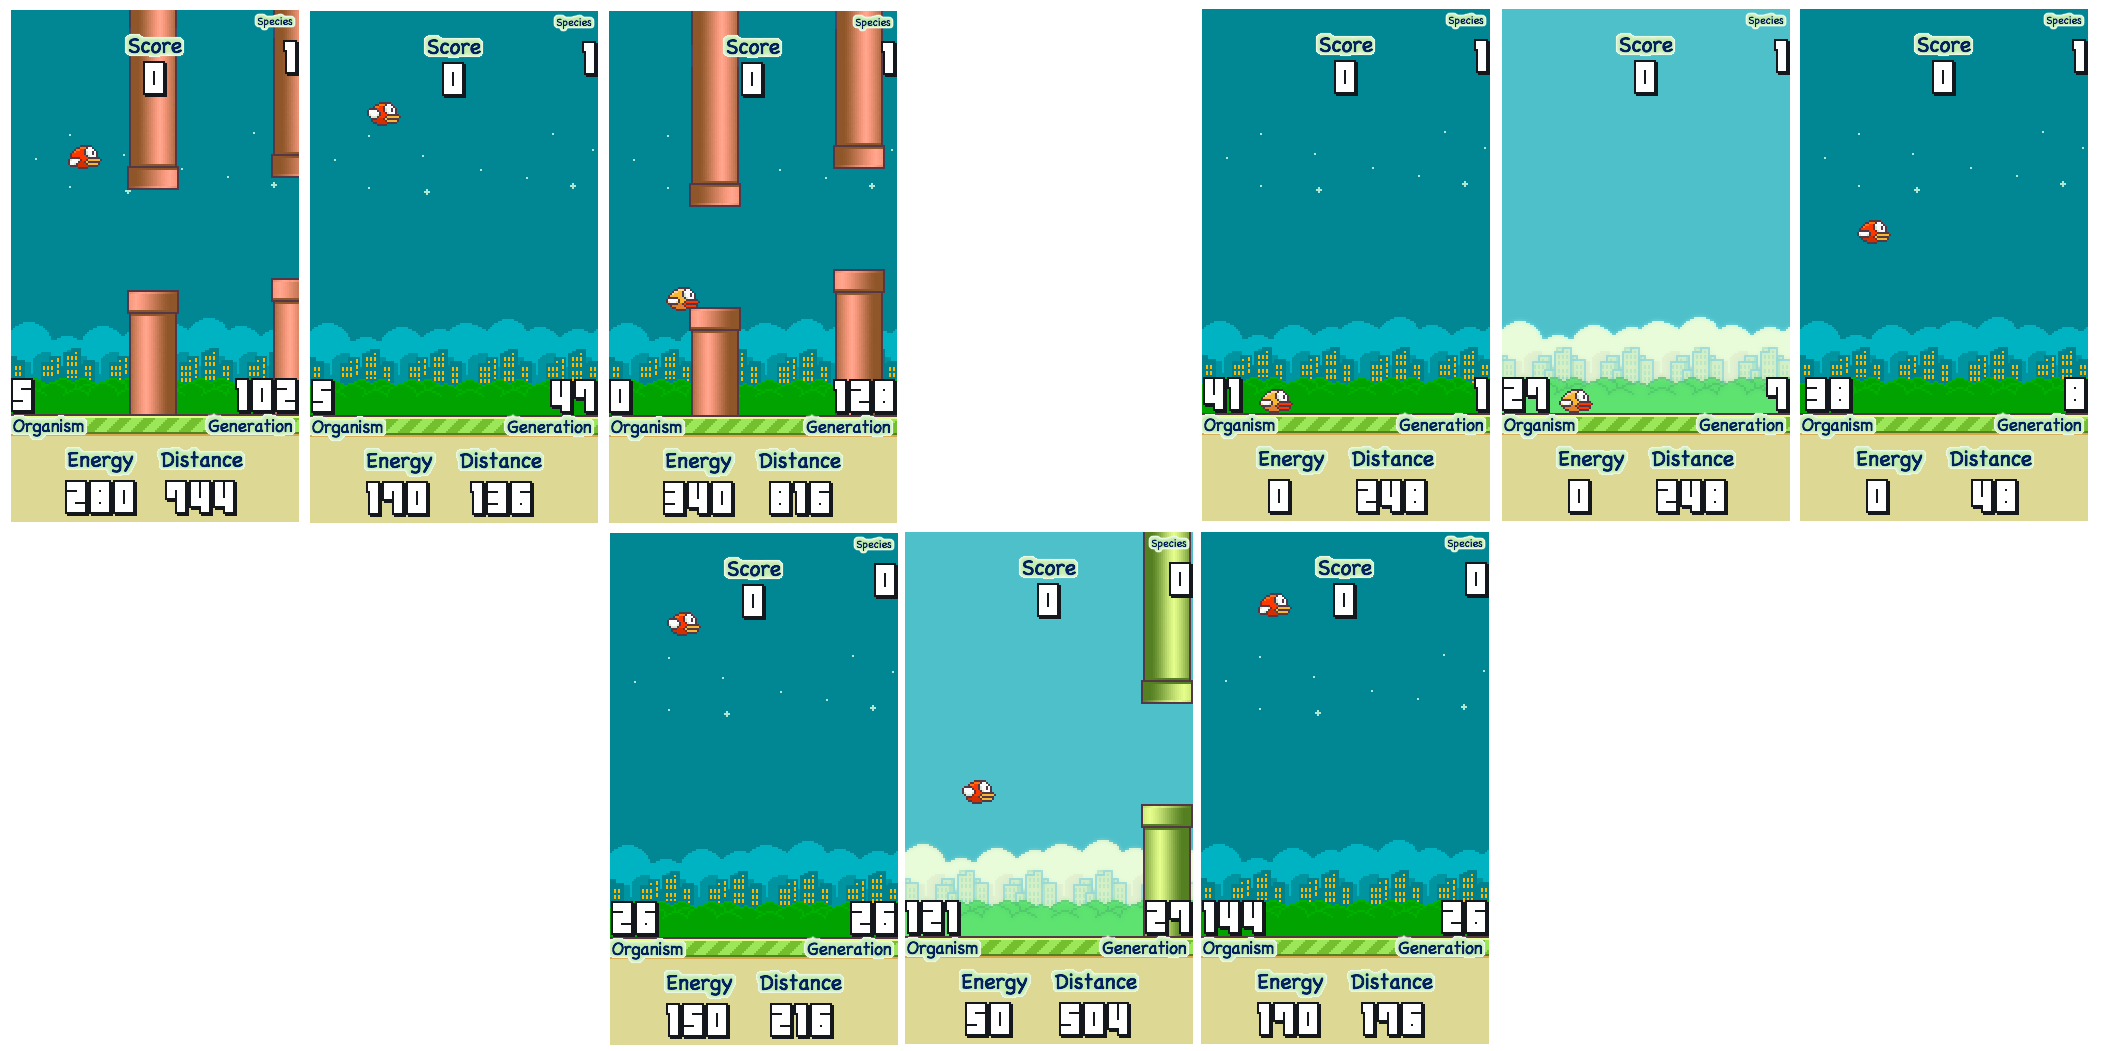
\includegraphics[width=1\textwidth]{graphics/flappy/flappy_sim_s1}
			\caption{Flappy Birds simulation}
		\end{figure}
		
		\begin{enumerate}
			\item explanation of environment and expectations
			\item fitnessfunction, formlar?
			\item explanation of graph of population (10, 50, 250) averaged on generations (30 generations evenly choosen [equal spaces between generation numbers])  (abstract explanation)
			\item check if expectations of marI/O can confirm
			\item huge difference between best runs and majority of runs (extreme luck), => double graph
			\item Differences between runs 
			\item unexpectedly bad results
			\item => Neat vs other machine learning
			\begin{enumerate}
				\item Differences between runs (lucky runs with 4th champion generation)
			\end{enumerate}
		\end{enumerate}
		
		\paragraph{Population 10 / Generation 500}
			asdf
%			\begin{figure}[h!]
%				\centering
%				\begin{minipage}{0.33\textwidth}
%					\centering
%					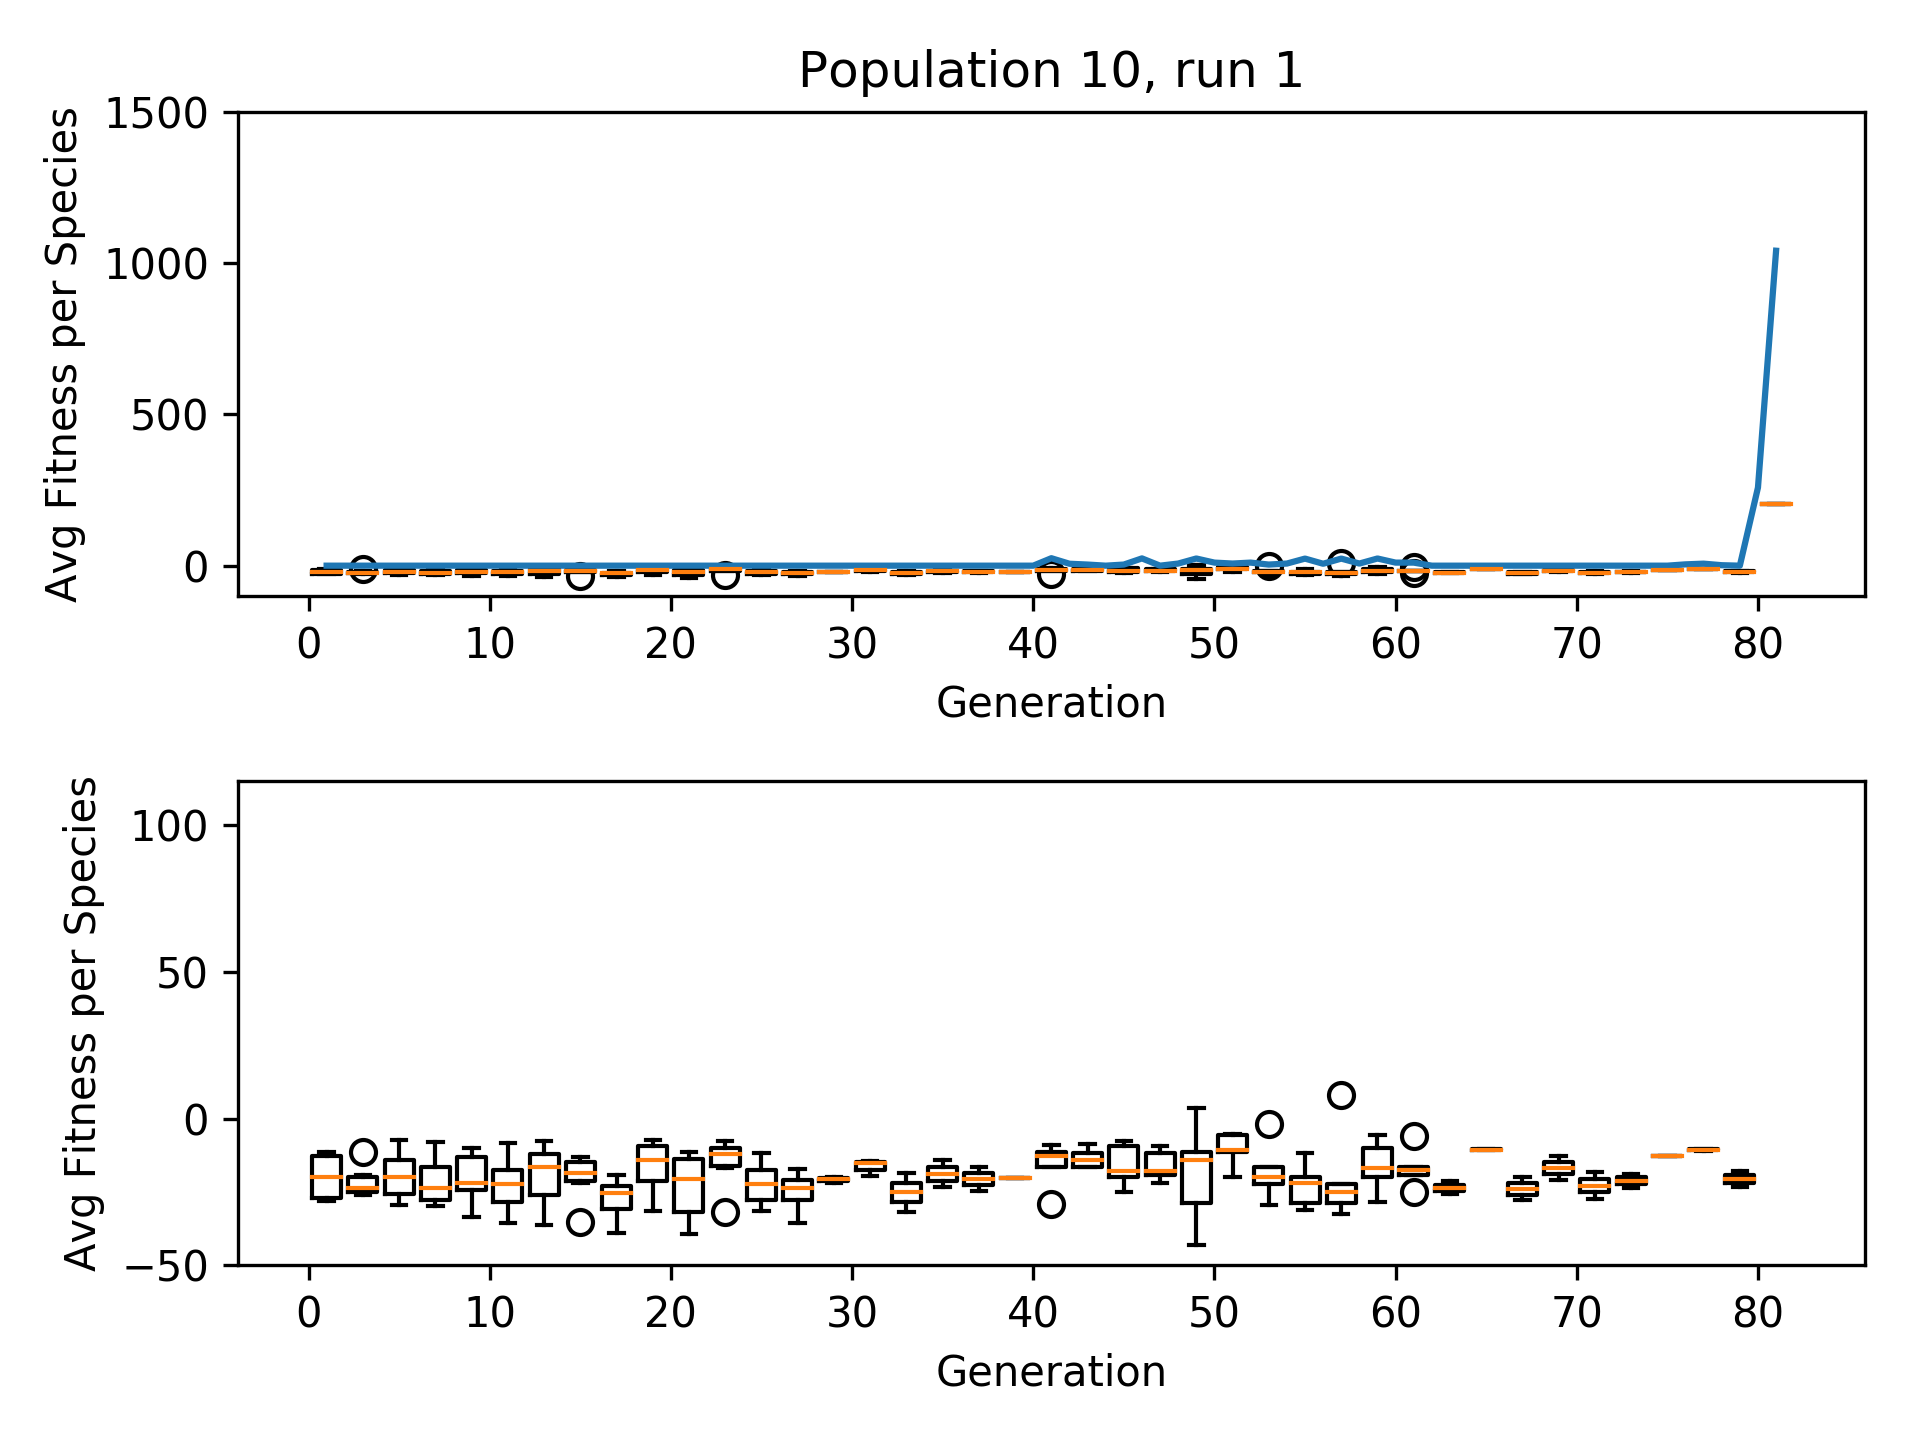
\includegraphics[width=1\textwidth]{graphics/flappy/pop10_run1} % first figure itself
%				\end{minipage}\hfill
%				\begin{minipage}{0.33\textwidth}
%					\centering
%					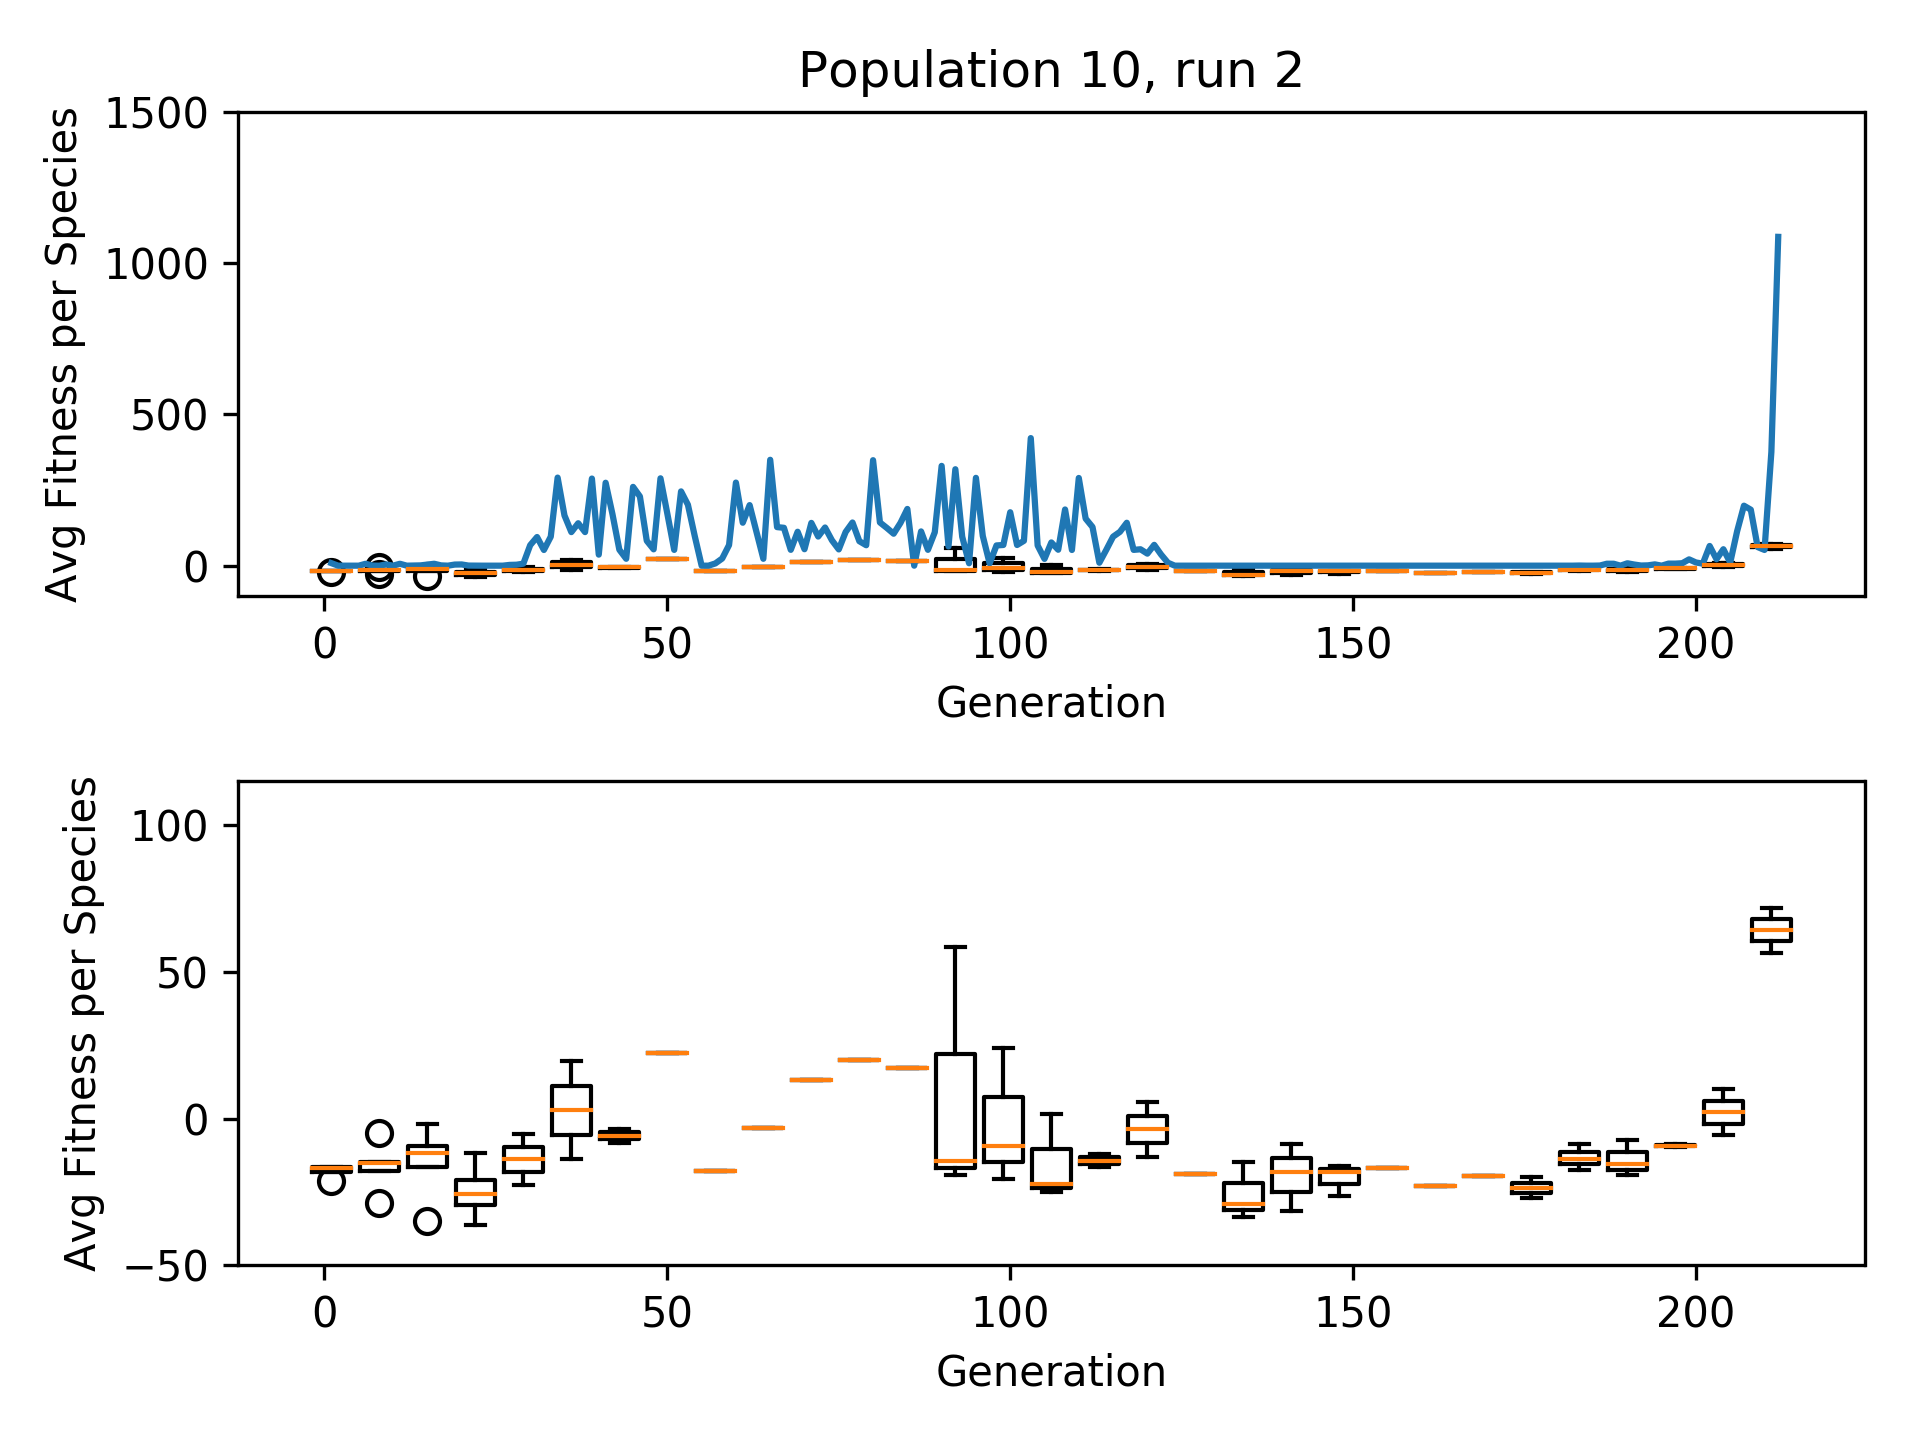
\includegraphics[width=1\textwidth]{graphics/flappy/pop10_run2} % second figure itself
%				\end{minipage}
%				\begin{minipage}{0.33\textwidth}
%					\centering
%					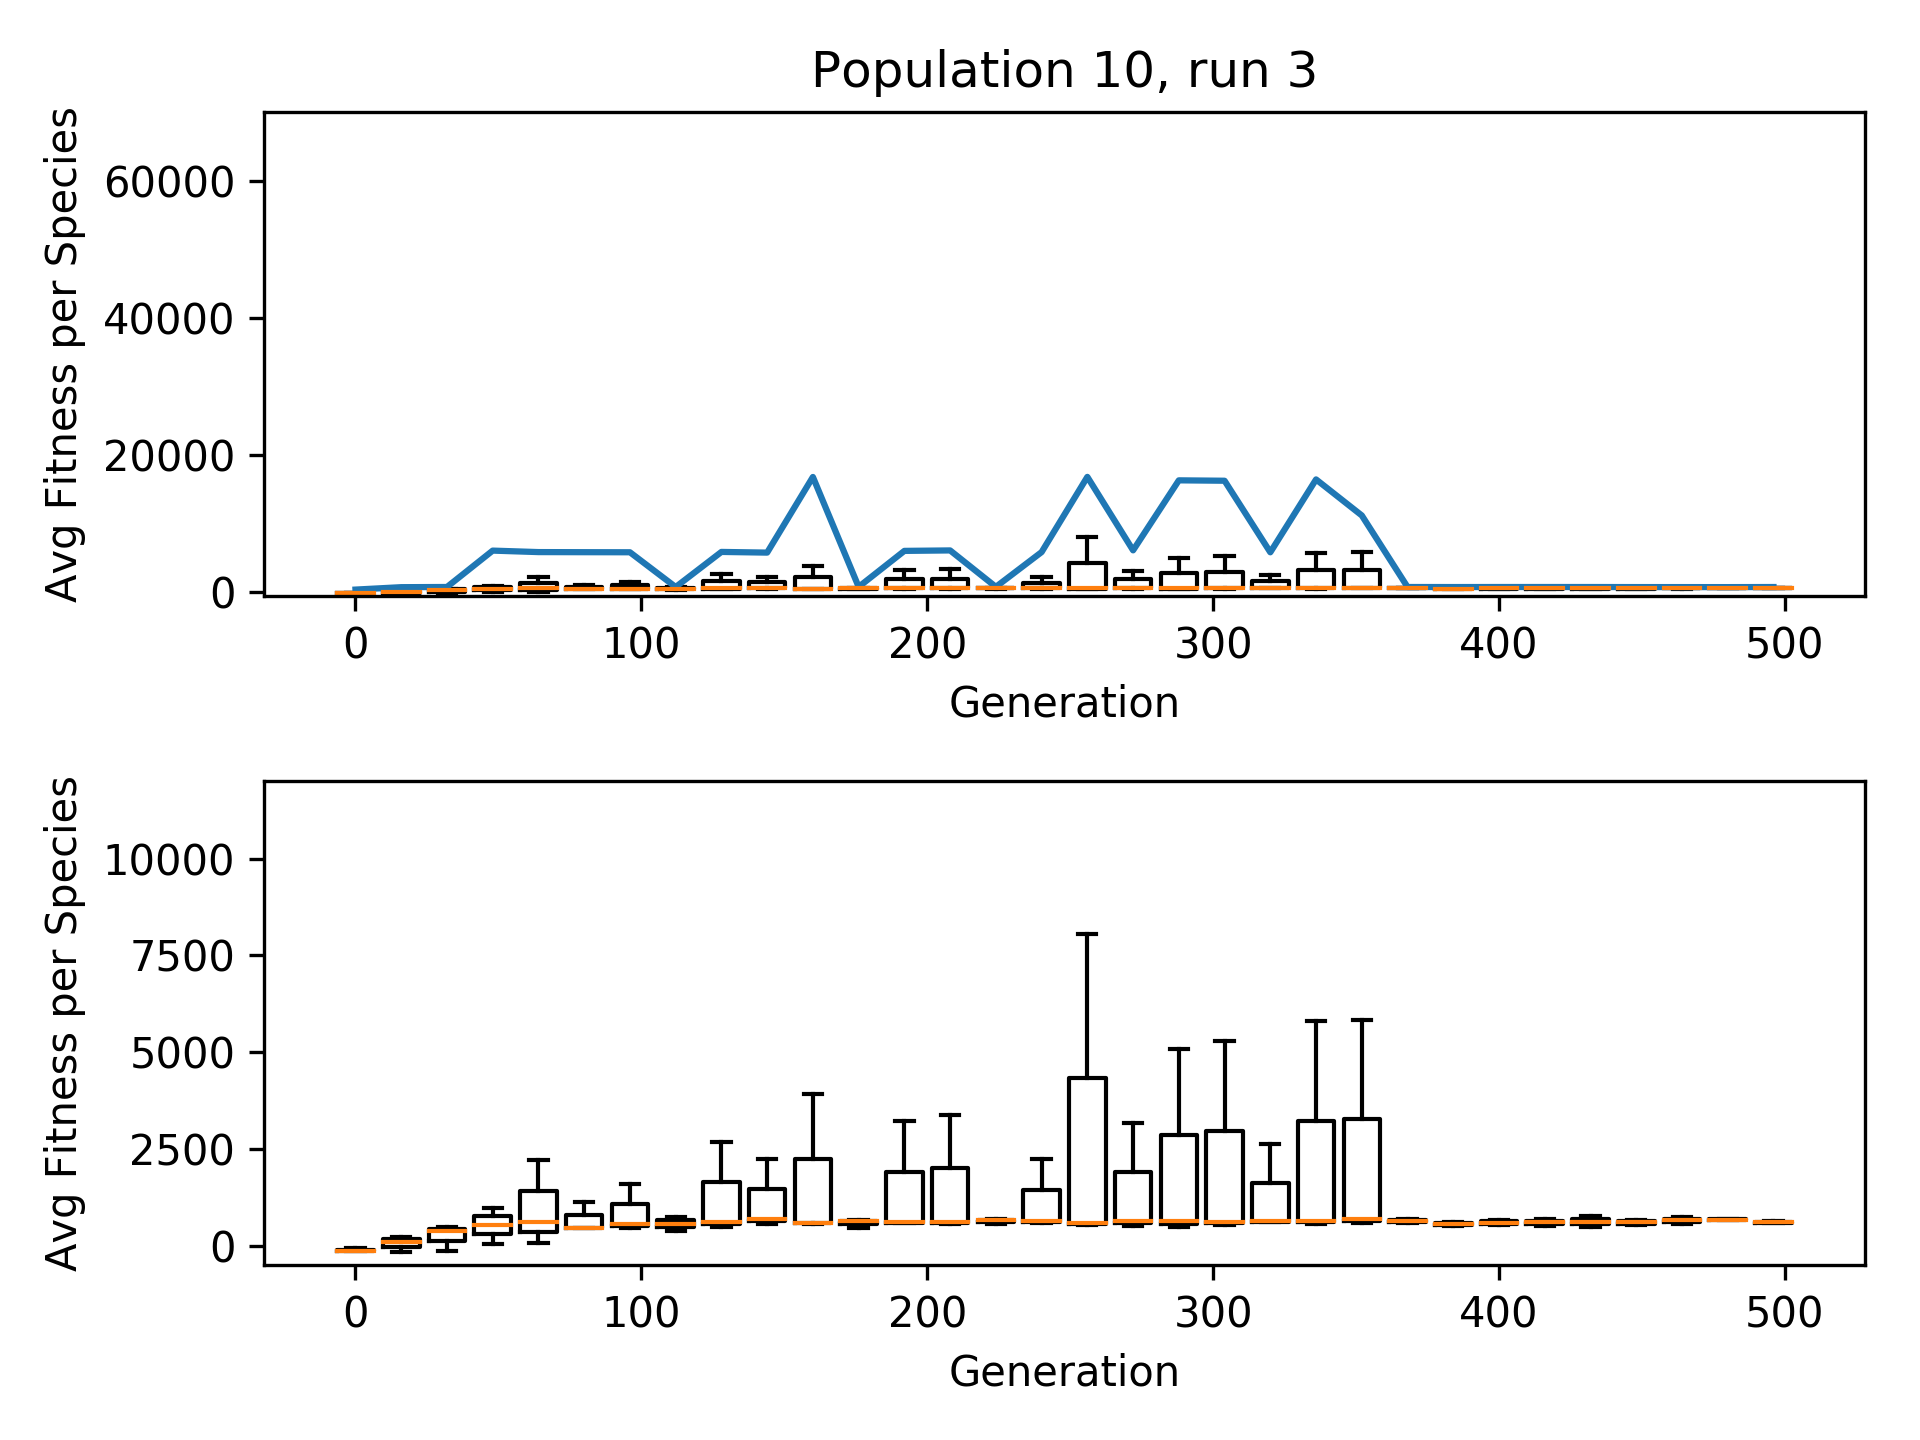
\includegraphics[width=1\textwidth]{graphics/flappy/pop10_run3} % second figure itself
%				\end{minipage}
%				\caption{Flappy Bird Population 10}
%			\end{figure}
		
		\paragraph{Population 50 / Generation 100}
			a
%			\begin{figure}[h]
%				\centering
%				\begin{minipage}{0.33\textwidth}
%					\centering
%					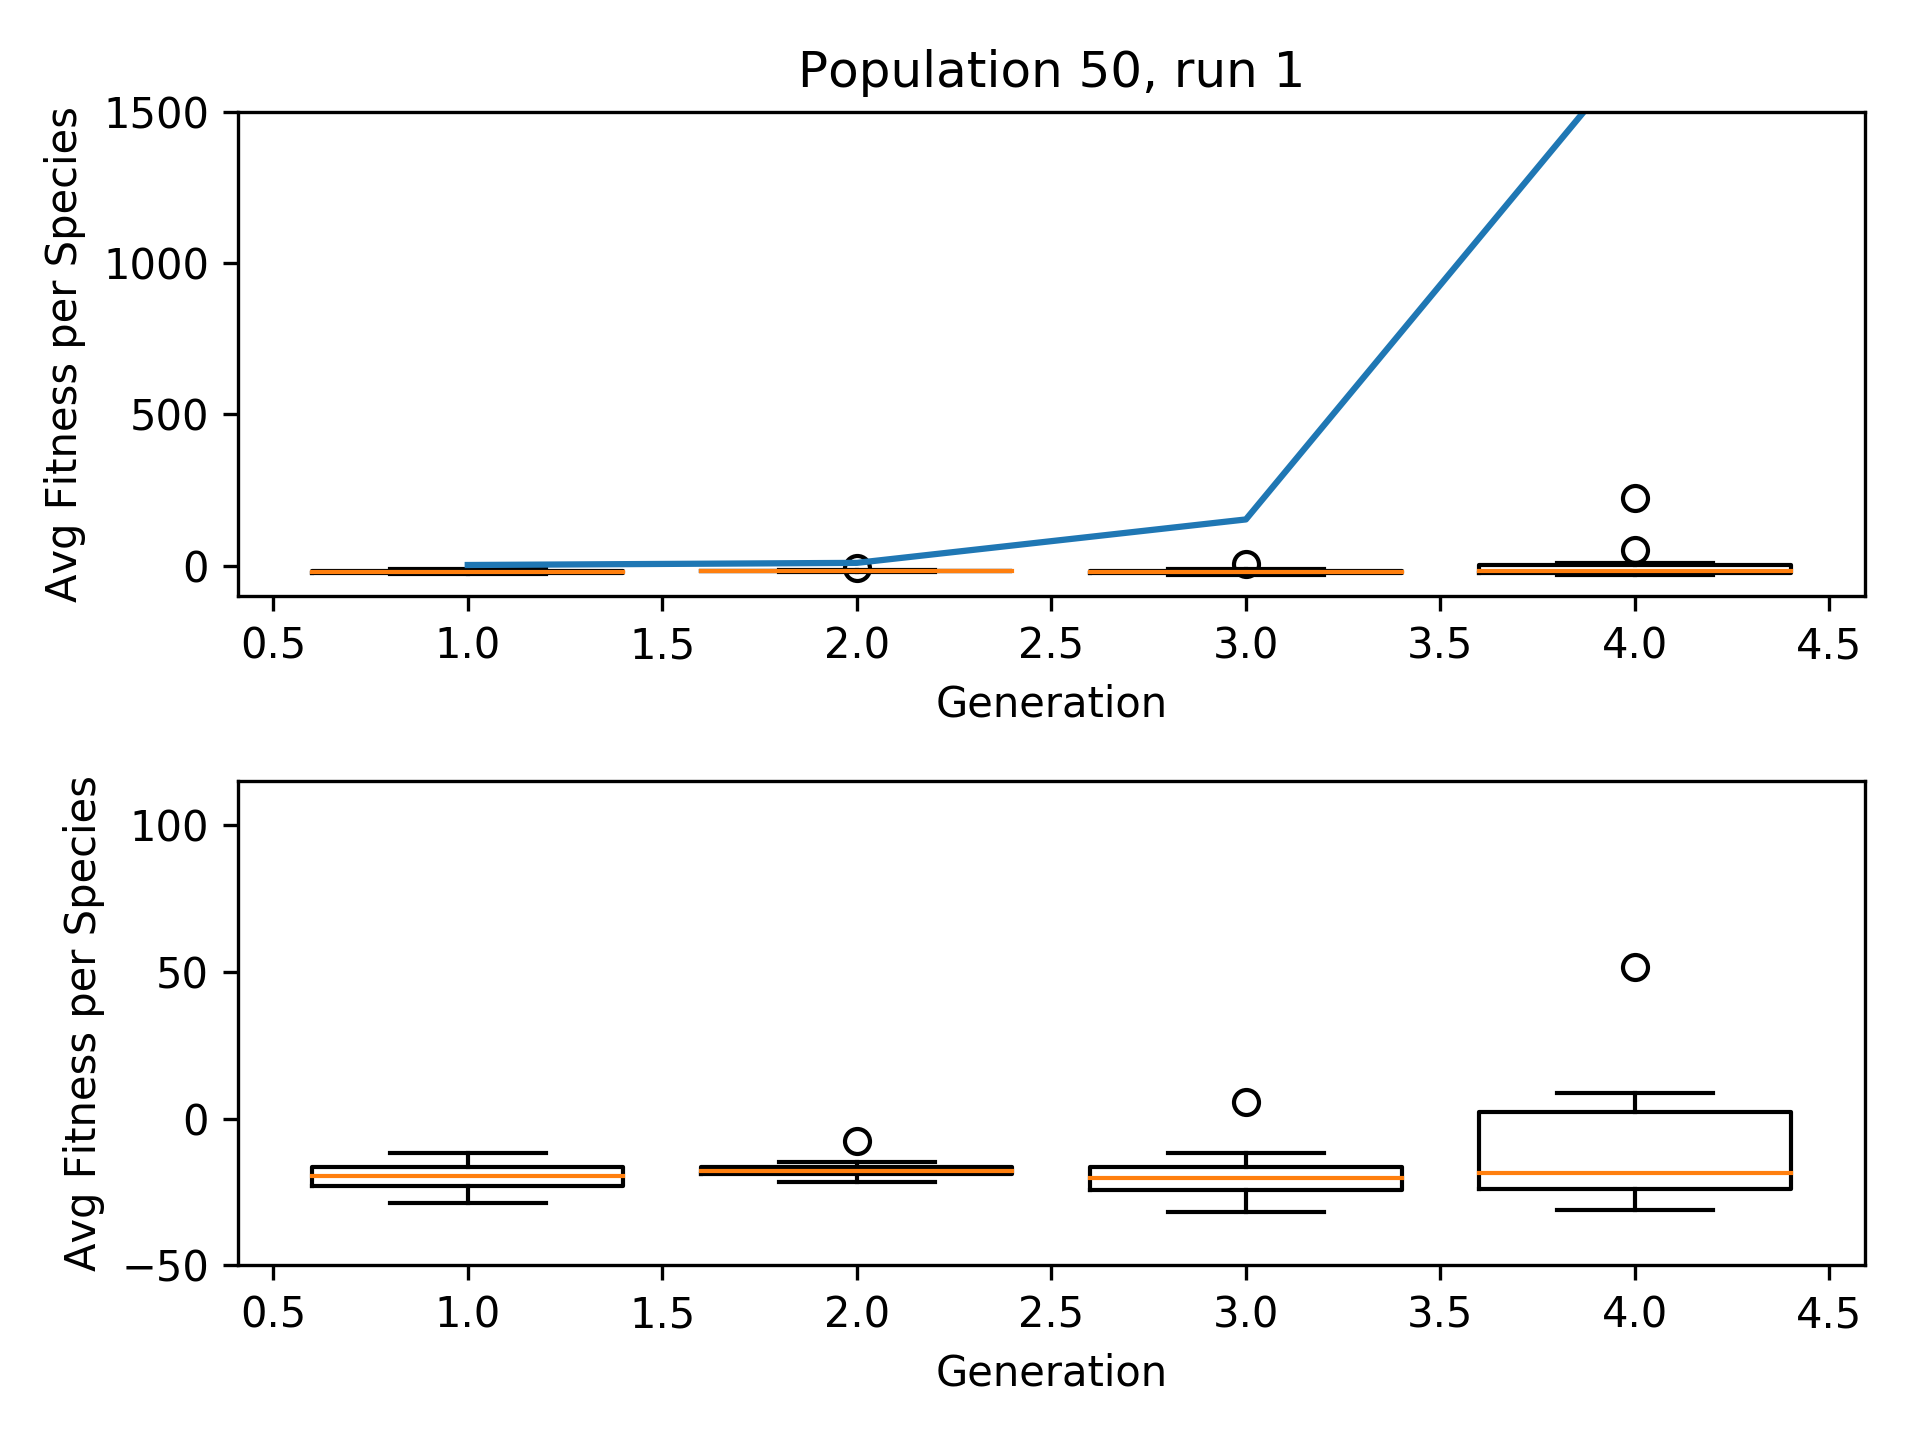
\includegraphics[width=1\textwidth]{graphics/flappy/pop50_run1} % first figure itself
%				\end{minipage}\hfill
%				\begin{minipage}{0.33\textwidth}
%					\centering
%					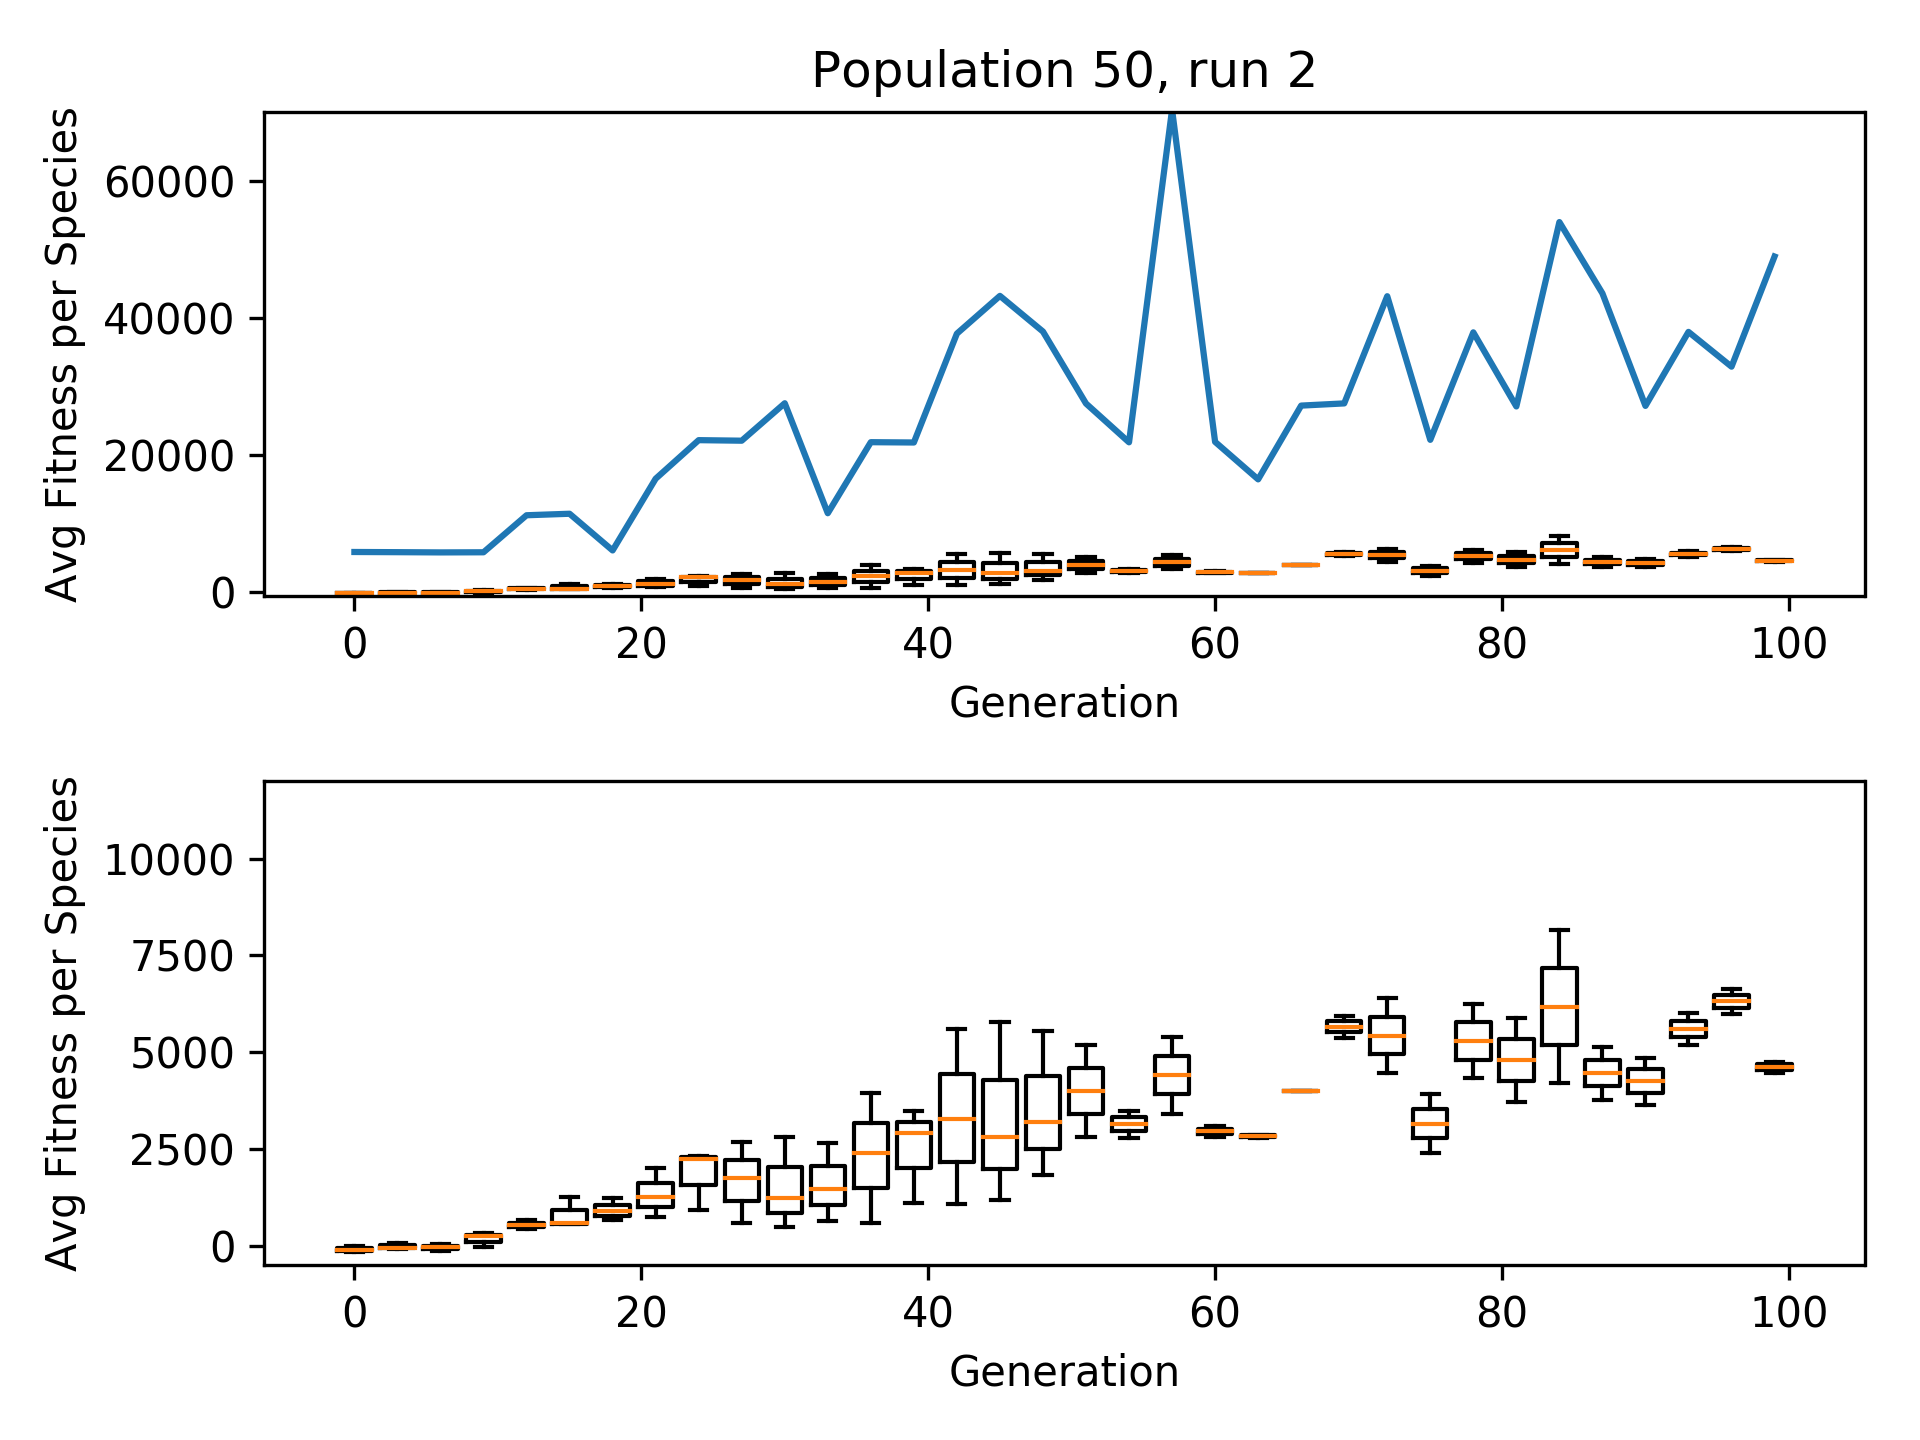
\includegraphics[width=1\textwidth]{graphics/flappy/pop50_run2} % second figure itself
%				\end{minipage}
%				\begin{minipage}{0.33\textwidth}
%					\centering
%					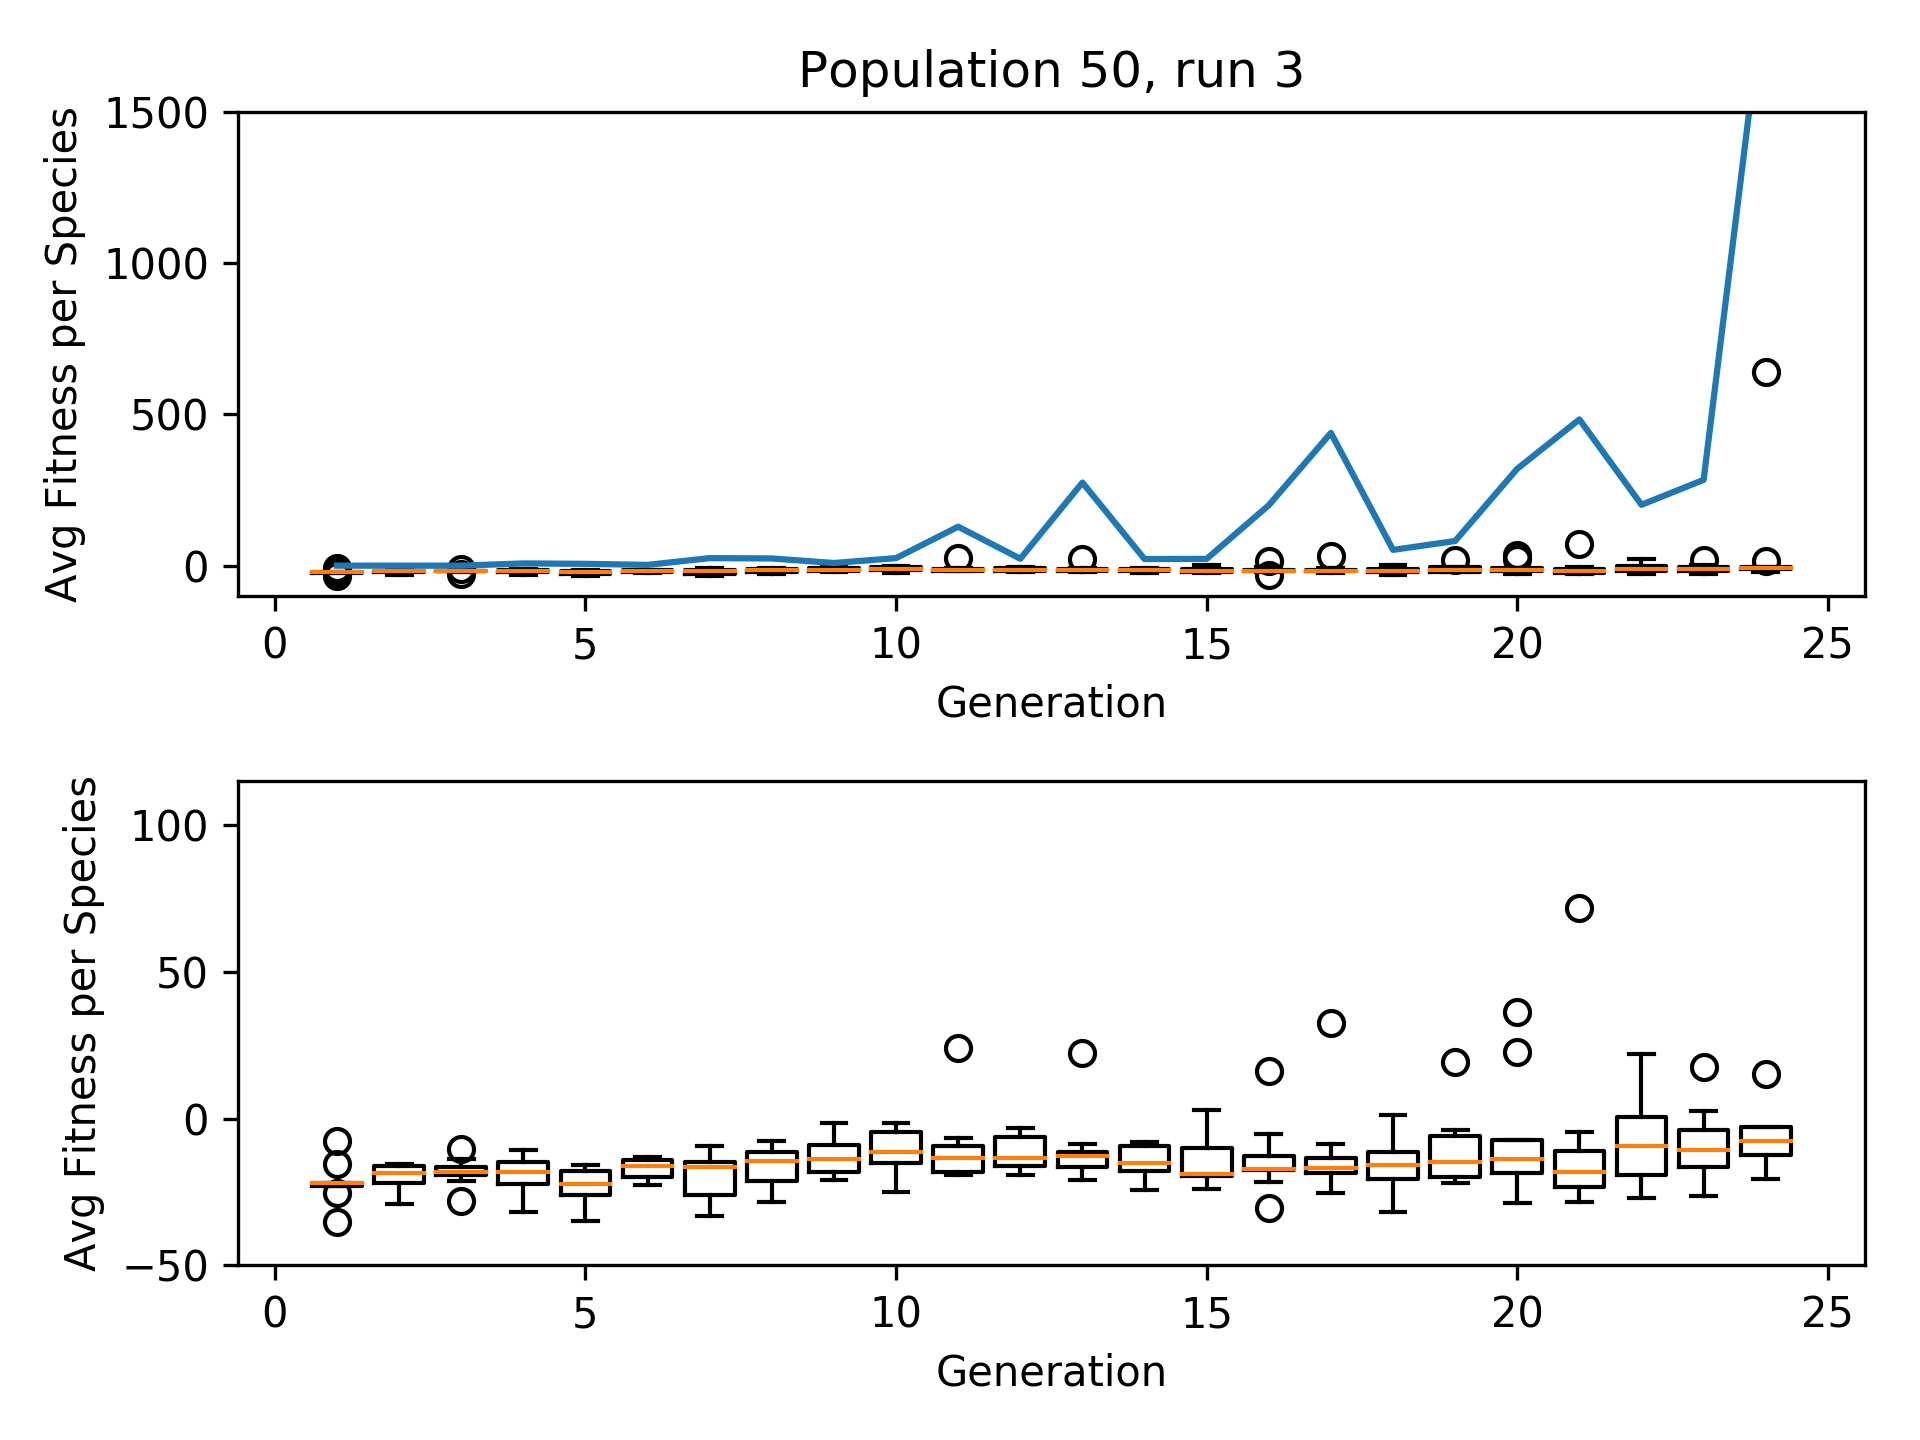
\includegraphics[width=1\textwidth]{graphics/flappy/pop50_run3} % second figure itself
%				\end{minipage}
%				\caption{Flappy Bird Population 50}
%			\end{figure}
		
		\paragraph{Population 250 / Generation 30}
		
			\begin{enumerate}
				\item best runs are exceptions (outside of whiskers)
			\end{enumerate}
			
%			\begin{figure}[h]
%				\centering
%				\begin{minipage}{0.33\textwidth}
%					\centering
%					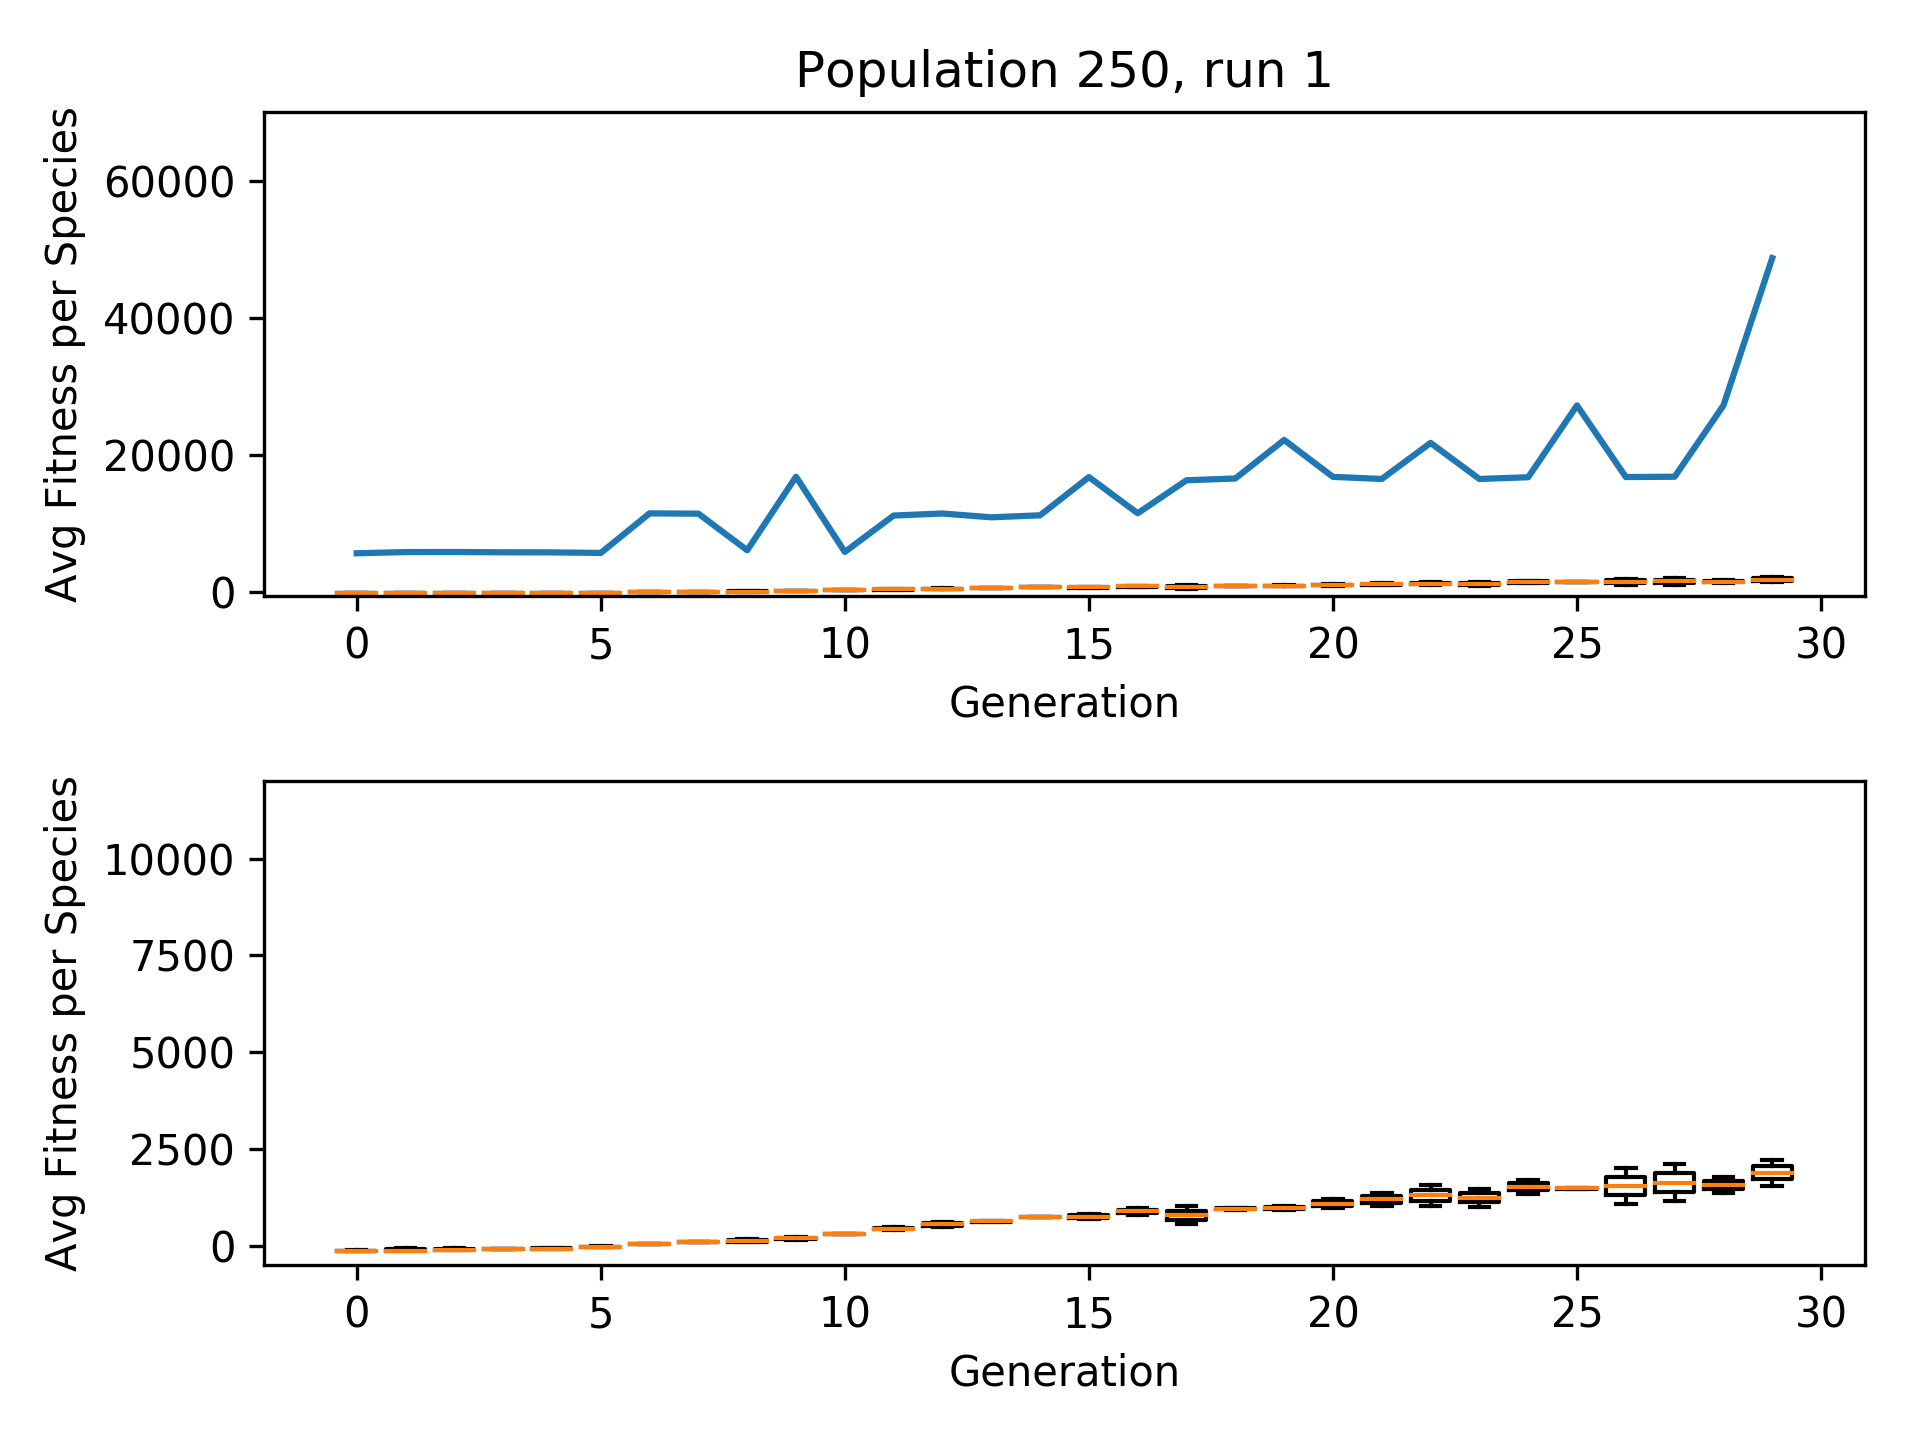
\includegraphics[width=1\textwidth]{graphics/flappy/pop250_run1} % first figure itself
%				\end{minipage}\hfill
%				\begin{minipage}{0.33\textwidth}
%					\centering
%					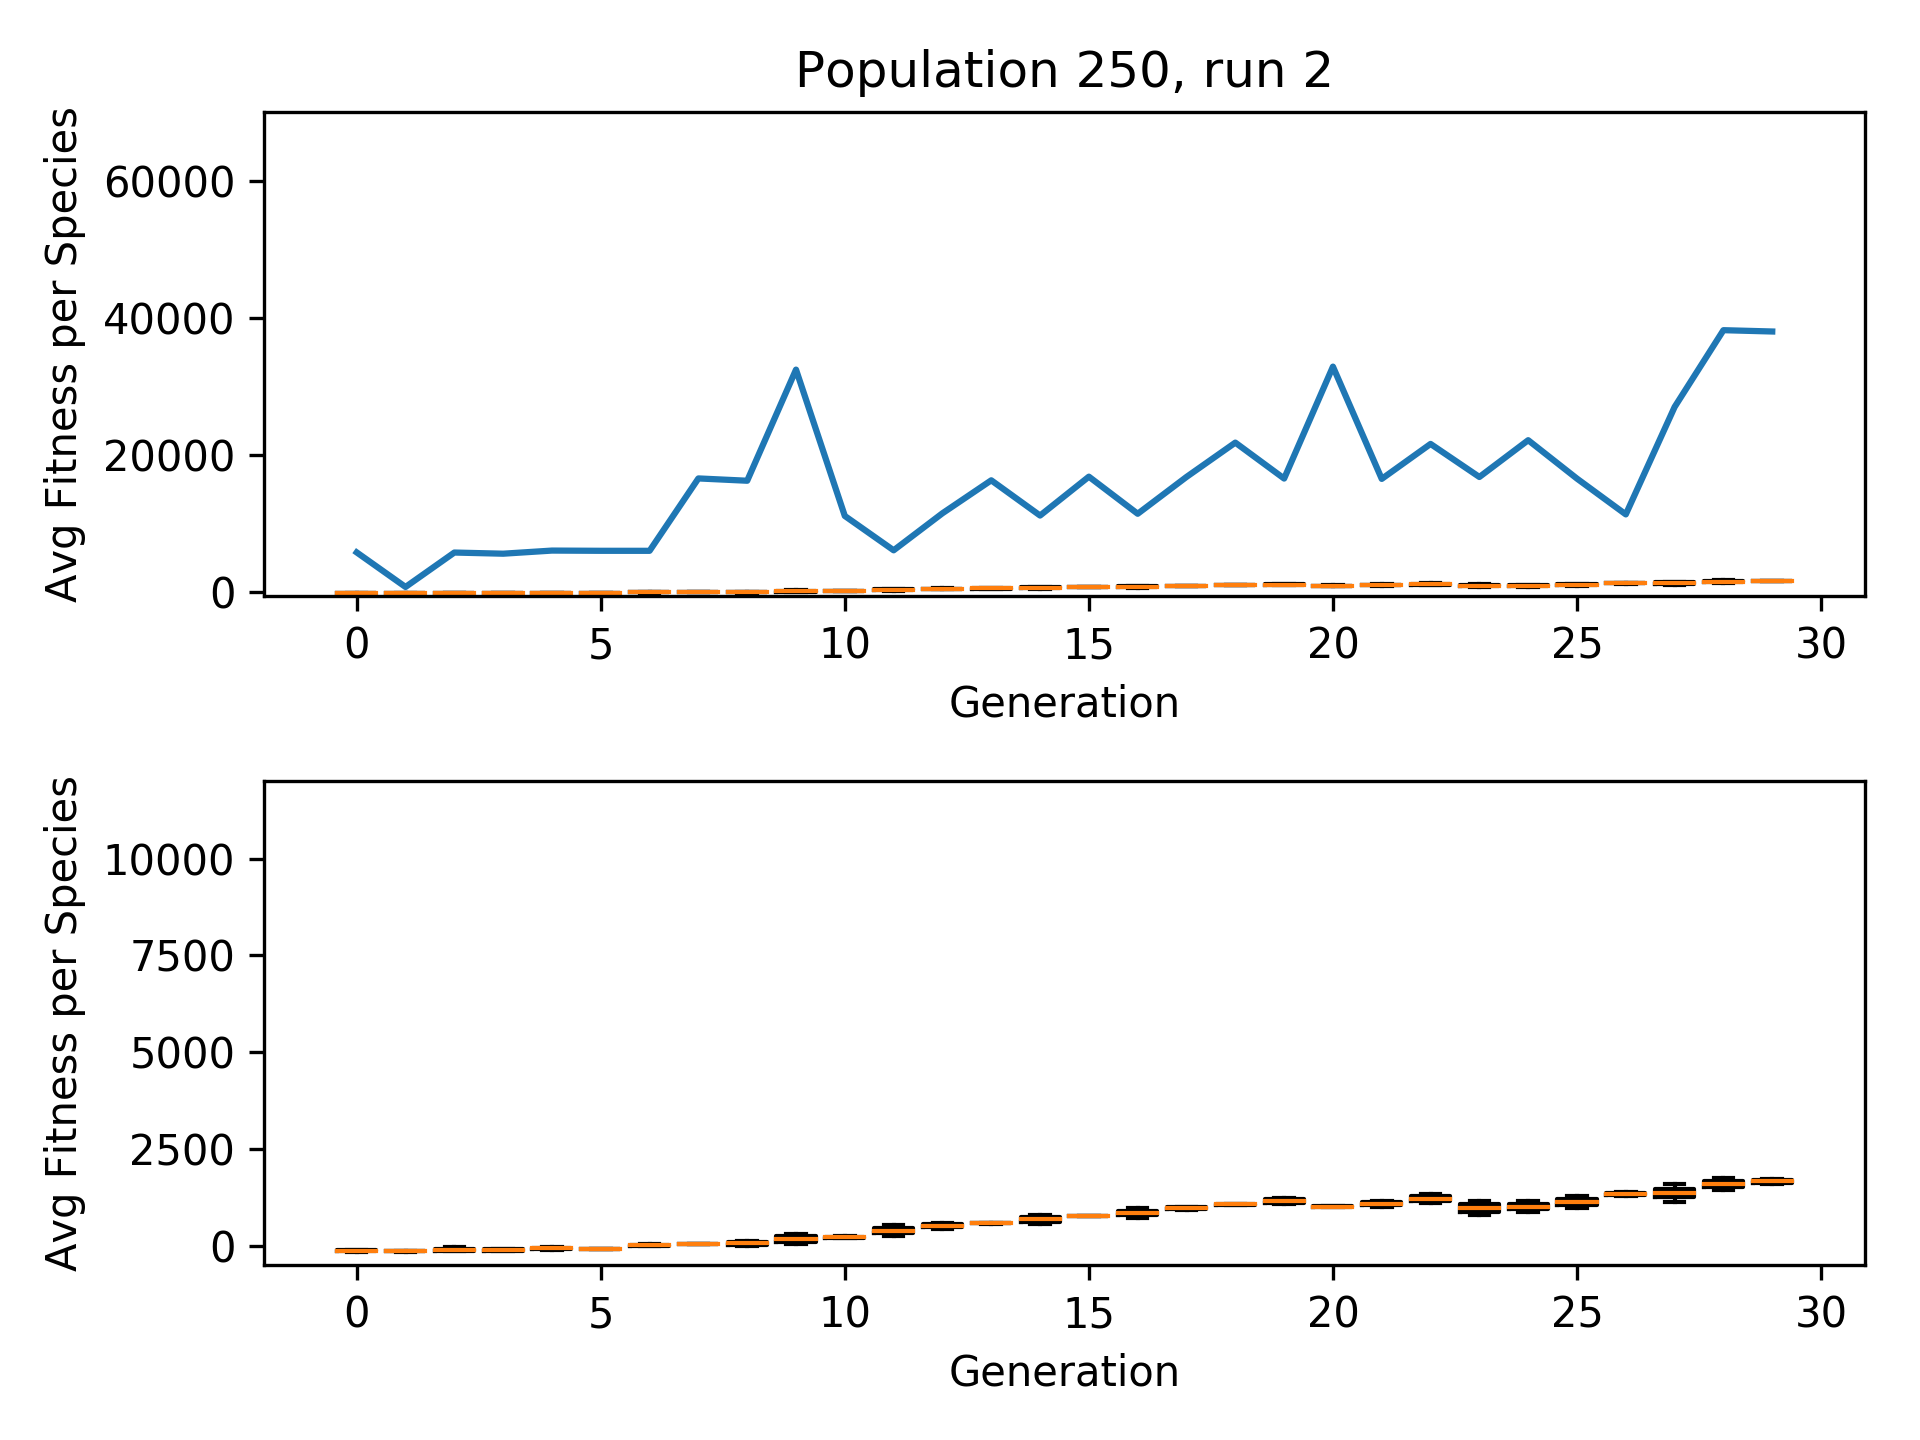
\includegraphics[width=1\textwidth]{graphics/flappy/pop250_run2} % second figure itself
%				\end{minipage}
%				\begin{minipage}{0.33\textwidth}
%					\centering
%					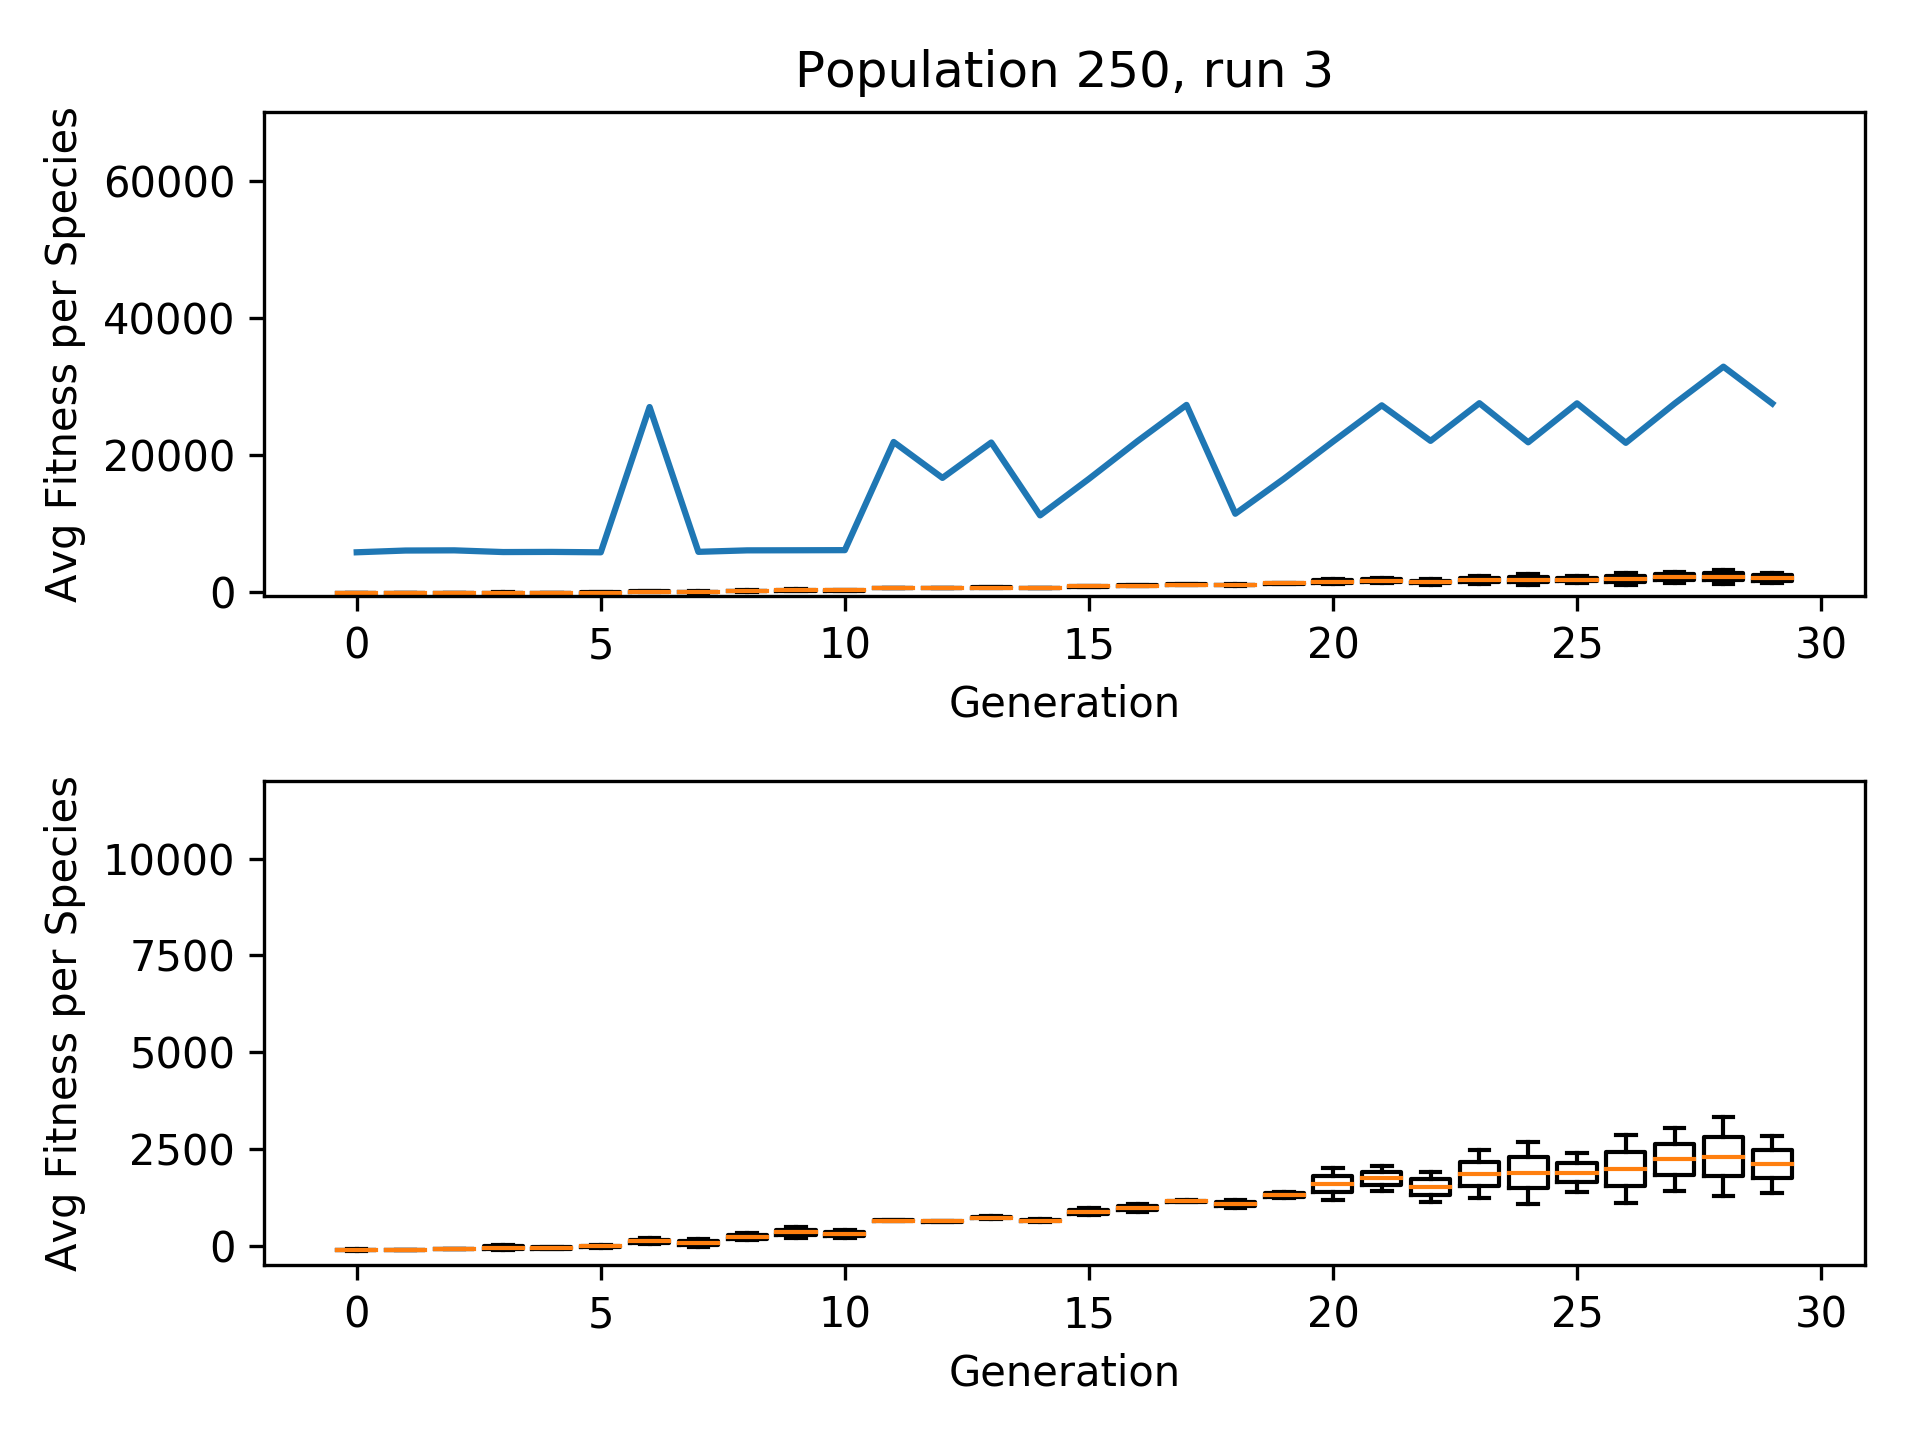
\includegraphics[width=1\textwidth]{graphics/flappy/pop250_run3} % second figure itself
%				\end{minipage}
%				\caption{Flappy Bird Population 250}
%			\end{figure}
		
		
		\subsection{Plain Machine learning flappy bird}
			\begin{enumerate}
				\item better results
				\item multi simulation made it easier
				\item easy algorithm for easy environment might be explanation for better results
			\end{enumerate}
	
	
	\section{Conclusion}
		\label{sec:system:conclusion}
		\begin{enumerate}
			\item differences / similarities in implementation (fixed size in machine learning flappy bird whereas dynamic species with marI/O)
			\item differences / similarities in outcome
			\item future studies
				\begin{itemize}
					\item genome/generation plot \& differences to other plot
					\item check in text for (future or further)
				\end{itemize}
		\end{enumerate}

         % INCLUDE: system
% !TEX root = ../thesis.tex


\chapter{Comparison and Meta-Analysis}
\label{sec:compare}

Much data was gathered and now we want to find out what this data indicates and how it can be used for future projects, maybe even real-world applications. 

\paragraph{Ignored Parameters}
\label{sec:compare:params}	
	In order to find a straight line for analyzing the data, many parameters were set by their default value. Other parameters have abstract meanings or simply define boundaries that didn't have to be considered. For example, in the configuration file of the \gls{neat} framework used in NEAT\_FlappyBird there are 63 lines of configuration.\\
	This complex set-up of the games leaves many wheels to turn and also give space to study their effect on the results systematically in future works. One starting-point can be the \gls{nn} parameters that were pre-specified for this simulations.\\
	Furthermore, the \gls{neat} implementations were not equal. First of all, they were written in two different programming/scripting languages. Furthermore, MarI/O was written from scratch and NEAT\_FlappyBird used a \gls{neat}-framework that allowed a high level of set-up-configurations and even self-implementations for various aspects of the algorithm. In this application only the default implementations were used as indicated by the following config initialization:
	\lstset{style=myPythonstyle} 
	\begin{lstlisting}[basicstyle=\small]
	config = neat.Config(neat.DefaultGenome, neat.DefaultReproduction, 
	neat.DefaultSpeciesSet, neat.DefaultStagnation, "config") 
	\end{lstlisting}
	However, despite the different set-up and configuration some similar results could be achieved using the \gls{neat} algorithm:

\section{Comparison of the different game environment}
\label{sec:compare:compare}	
	However, one parameter that was manipulated for this analyses is the initial population size. In MarI/O the initial population size spawned the defined amount of species with one genome each. In flappy bird, however, there were as many genomes launched as defined by the population size and after the run, they got assigned to their species.\\
	In order to display the differences in an overview, a table is presented containing the data trends. Despite their similarity, different fitness-functions have been taken to evaluate the success of a genome. This results in different scales in their values. That's why a more abstract indicator of the trend was chosen instead of the numbers. An arrow up ($\Big\uparrow$) indicates that the value was rising with a bigger initial population size and an arrow down ($\Big\downarrow$) indicates the opposite. When there is an $\bigtimes$ shown, it means that no trend could be found within the three population classes.
	\begin{table}[h]
		\centering
		\resizebox{\textwidth}{!}{
			\begin{tabular}[width=0.5\textwidth]{@{}ll|l|l|l|l@{}}
				\toprule
				Data Trend Comparison		& avg. runs /$\sigma$ 			& avg. fitness score /$\sigma$ 		& avg distance /$\sigma$ 		& avg. regress /$\sigma$ 			& avg. fitness increase /$\sigma$ 	\\ \midrule
				{\Large MarI/O} 			& $\Big\uparrow$ /$\times$      & $\Big\downarrow$ /$\downarrow$ 	& $\Big\uparrow$ /$\times$  	& $\Big\downarrow$ /$\downarrow$    & $\Big\uparrow$ /$\times$          \\
				{\Large NEAT\_FlappyBird}	& $\bigtimes$ /$\downarrow$    	& $\bigtimes$ /$\downarrow$ 		& $\Big\uparrow$ /$\times$  	& $\bigtimes$ /$\times$    			& $\Big\uparrow$ /$\times$          \\ \bottomrule
			\end{tabular}
		}
		\caption{Date Trend Comparison of different games and their \gls{neat} implementation}
		\label{tab:comp}
	\end{table} 
	At first, the differences are pointed out which are the following: 
	In MarI/O the average fitness score dropped with a bigger initial population. In NEAT\_FlappyBird there couldn't be a correlation drawn between the population size and the average fitness score.\\
	However, the standard deviation of the average fitness score dropped in both environments. This outcome is reasonable since there are fewer generations when the initial population size is larger.\\
	Further, in MarI/O the average regress (if present) becomes lower with bigger population sizes, as well as it's deviation. Interestingly, in NEAT\_FlappyBird no trend could be found at all since the population class had a higher average regress than the population class 10 but population class 250 didn't have any regress at all.\\
	The standard deviation of the average fitness increase had no trend in the NEAT\_FlappyBird implementation, however, it was quite similar in MarI/O's simulations. Still, the trend of the average fitness increase is the same in both simulations.
	
	When looking at the similarities of the results of the two environments there are two trends visible:
	One not so obvious correlation is that the distance of the median of the species to the best run of each generation is becoming greater with a greater population count. However, the standard deviation of this data is quite high in some cases. Still, in population class 250, the standard deviation was low when compared to the average regress value in MarI/O as well as NEAT\_FlappyBird.\\
	A more reasonable trend is that the population class 250 has a bigger average fitness increase than the other two simulation classes since the number of generations are smaller, although the goal/threshold was reached as well.\\
	When comparing the average distance with the average fitness increase, it can be seen that there are only a few genomes in the runs of population class 250 that reached a higher score, however, the majority of runs remained low. This division becomes larger the bigger the initial population size is. In MarI/O the average regress became lower with a higher population count, which indicates a certain stability. However, this stability could not be found in Flappy Bird. A reason for this can be the known bad performance of neat in extreme situations, since Flappy Bird has a randomly generated and therefore unknown world, whereas Super Mario World is deterministic in its level behavior\cite{kohl_integrated_2011}.
       % INCLUDE: concepts
% !TEX root = ../thesis.tex
%
\chapter{Conclusion}
\label{sec:conclusion}

\chapterprecishere{"By far, the greatest danger of Artificial Intelligence is that people conclude too early that they understand it."\par\raggedleft--- \textup{Eliezer S. Yudkowsky}, (Artificial Intelligence Researcher)}

% \cleanchapterquote{By far, the greatest danger of Artificial Intelligence is that people conclude too early that they understand it.}{Eliezer S. Yudkowsky}{(Artificial Intelligence Researcher)}

https://sokogskriv.no/en/writing/structure/structuring-a-thesis/
http://www.charleslipson.com/How-to-write-a-thesis.htm

\begin{itemize}
	\item 
	\item test MarI/O previous evolutions on other levels (long: what would be expected, how long to adapt to differences, would be better than start from anew)
	\item compare MarI\O to other solutions (see paper unofficial paper https://www.cs.cmu.edu/~tom7/mario/mario.pdf)
\end{itemize}


\section{Stuff}
\label{sec:conclusion:sec1}


\section{Future Work}
\label{sec:conclusion:future}

     % INCLUDE: conclusion

% --------------------------
% Back matter
% --------------------------
\appendix\cleardoublepage
% !TEX root = ../my-thesis.tex
%
\chapter{Example Appendix}
\label{sec:appendix}


\section{Appendix Section 1}
\label{sec:appendix:sec1}

\begin{table}[h]
	\begin{tabularx}{\textwidth}{X | X | X}
		%\hline
		Alpha		& Beta			& Gamma			\\ \hline
		0			& 1				& 2				\\ \hline
		3			& 4				& 5				\\ %\hline
	\end{tabularx}
	\label{tab:table1}
	\caption{This is a caption text.}
\end{table}

       % INCLUDE: appendix
%
{%
\setstretch{1.1}
\renewcommand{\bibfont}{\normalfont\small}
\setlength{\biblabelsep}{0pt}
\setlength{\bibitemsep}{0.5\baselineskip plus 0.5\baselineskip}
\printbibliography[nottype=online]
\printbibliography[heading=subbibliography,title={Webpages},type=online,prefixnumbers={@}]
}
\cleardoublepage

\listoffigures
\cleardoublepage

\listoftables
\cleardoublepage

\input{content/declaration}
\clearpage
\newpage
\mbox{}

% **************************************************
% End of Document CONTENT
% **************************************************
\end{document}
